\documentclass[12pt]{article}
\usepackage[english]{babel}
\usepackage[utf8]{inputenc}
\usepackage[english]{babel}
\usepackage[a4paper, total={7.25in, 9.5in}]{geometry}
\usepackage{tikz-feynman}
\tikzfeynmanset{compat=1.0.0} 
\usepackage{subcaption}
\usepackage{float}
\floatplacement{figure}{H}
\usepackage{simpler-wick}
\usepackage{mathrsfs}  
\usepackage{dsfont}
\usepackage{relsize}
\usepackage{tikz-cd}
\DeclareMathAlphabet{\mathdutchcal}{U}{dutchcal}{m}{n}

\usepackage{cancel}



\newcommand{\field}{\hat{\Phi}}
\newcommand{\dfield}{\hat{\Phi}^\dagger}
 
\usepackage{amsthm, amssymb, amsmath, centernot}
\usepackage{slashed}
\newcommand{\notimplies}{%
  \mathrel{{\ooalign{\hidewidth$\not\phantom{=}$\hidewidth\cr$\implies$}}}}
 
\renewcommand\qedsymbol{$\square$}
\newcommand{\cont}{$\boxtimes$}
\newcommand{\divides}{\mid}
\newcommand{\ndivides}{\centernot \mid}

\newcommand{\Integers}{\mathbb{Z}}
\newcommand{\Natural}{\mathbb{N}}
\newcommand{\Complex}{\mathbb{C}}
\newcommand{\Zplus}{\mathbb{Z}^{+}}
\newcommand{\Primes}{\mathbb{P}}
\newcommand{\Q}{\mathbb{Q}}
\newcommand{\R}{\mathbb{R}}
\newcommand{\ball}[2]{B_{#1} \! \left(#2 \right)}
\newcommand{\Rplus}{\mathbb{R}^+}
\renewcommand{\Re}[1]{\mathrm{Re}\left[ #1 \right]}
\renewcommand{\Im}[1]{\mathrm{Im}\left[ #1 \right]}
\newcommand{\Op}{\mathcal{O}}

\newcommand{\invI}[2]{#1^{-1} \left( #2 \right)}
\newcommand{\End}[1]{\text{End}\left( A \right)}
\newcommand{\legsym}[2]{\left(\frac{#1}{#2} \right)}
\renewcommand{\mod}[3]{\: #1 \equiv #2 \: \mathrm{mod} \: #3 \:}
\newcommand{\nmod}[3]{\: #1 \centernot \equiv #2 \: mod \: #3 \:}
\newcommand{\ndiv}{\hspace{-4pt}\not \divides \hspace{2pt}}
\newcommand{\finfield}[1]{\mathbb{F}_{#1}}
\newcommand{\finunits}[1]{\mathbb{F}_{#1}^{\times}}
\newcommand{\ord}[1]{\mathrm{ord}\! \left(#1 \right)}
\newcommand{\quadfield}[1]{\Q \small(\sqrt{#1} \small)}
\newcommand{\vspan}[1]{\mathrm{span}\! \left\{#1 \right\}}
\newcommand{\galgroup}[1]{Gal \small(#1 \small)}
\newcommand{\bra}[1]{\left| #1 \right>}
\newcommand{\Oa}{O_\alpha}
\newcommand{\Od}{O_\alpha^{\dagger}}
\newcommand{\Oap}{O_{\alpha '}}
\newcommand{\Odp}{O_{\alpha '}^{\dagger}}
\newcommand{\im}[1]{\mathrm{im} \: #1}
\renewcommand{\ker}[1]{\mathrm{ker} \: #1}
\newcommand{\ket}[1]{\left| #1 \right>}
\renewcommand{\bra}[1]{\left< #1 \right|}
\newcommand{\inner}[2]{\left< #1 | #2 \right>}
\newcommand{\expect}[2]{\left< #1 \right| #2 \left| #1 \right>}
\renewcommand{\d}[1]{ \mathrm{d}#1 \:}
\newcommand{\dn}[2]{ \mathrm{d}^{#1} #2 \:}
\newcommand{\deriv}[2]{\frac{\d{#1}}{\d{#2}}}
\newcommand{\nderiv}[3]{\frac{\dn{#1}{#2}}{\d{#3^{#1}}}}
\newcommand{\pderiv}[2]{\frac{\partial{#1}}{\partial{#2}}}
\newcommand{\fderiv}[2]{\frac{\delta #1}{\delta #2}}
\newcommand{\parsq}[2]{\frac{\partial^2{#1}}{\partial{#2}^2}}
\newcommand{\topo}{\mathcal{T}}
\newcommand{\base}{\mathcal{B}}
\renewcommand{\bf}[1]{\mathbf{#1}}
\renewcommand{\a}{\hat{a}}
\newcommand{\adag}{\hat{a}^\dagger}
\renewcommand{\b}{\hat{b}}
\newcommand{\bdag}{\hat{b}^\dagger}
\renewcommand{\c}{\hat{c}}
\newcommand{\cdag}{\hat{c}^\dagger}
\newcommand{\hamilt}{\hat{H}}
\renewcommand{\L}{\hat{L}}
\newcommand{\Lz}{\hat{L}_z}
\newcommand{\Lsquared}{\hat{L}^2}
\renewcommand{\S}{\hat{S}}
\renewcommand{\empty}{\varnothing}
\newcommand{\J}{\hat{J}}
\newcommand{\lagrange}{\mathcal{L}}
\newcommand{\dfourx}{\mathrm{d}^4x}
\newcommand{\meson}{\phi}
\newcommand{\dpsi}{\psi^\dagger}
\newcommand{\ipic}{\mathrm{int}}
\newcommand{\tr}[1]{\mathrm{tr} \left( #1 \right)}
\newcommand{\C}{\mathbb{C}}
\newcommand{\CP}[1]{\mathbb{CP}^{#1}}
\newcommand{\Vol}[1]{\mathrm{Vol}\left(#1\right)}

\newcommand{\Tr}[1]{\mathrm{Tr}\left( #1 \right)}
\newcommand{\Charge}{\hat{\mathbf{C}}}
\newcommand{\Parity}{\hat{\mathbf{P}}}
\newcommand{\Time}{\hat{\mathbf{T}}}
\newcommand{\Torder}[1]{\mathbf{T}\left[ #1 \right]}
\newcommand{\Norder}[1]{\mathbf{N}\left[ #1 \right]}
\newcommand{\Znorm}{\mathcal{Z}}
\newcommand{\EV}[1]{\left< #1 \right>}
\newcommand{\interact}{\mathrm{int}}
\newcommand{\covD}{\mathcal{D}}
\newcommand{\conj}[1]{\overline{#1}}

\newcommand{\SO}[2]{\mathrm{SO}(#1, #2)}
\newcommand{\SU}[2]{\mathrm{SU}(#1, #2)}

\newcommand{\anticom}[2]{\left\{ #1 , #2 \right\}}


\newcommand{\pathd}[1]{\! \mathdutchcal{D} #1 \:}

\renewcommand{\theenumi}{(\alph{enumi})}


\renewcommand{\theenumi}{(\alph{enumi})}

\newcommand{\atitle}[1]{\title{% 
	\large \textbf{Physics GR8048 Quantum Field Theory II
	\\ Assignment \# #1} \vspace{-2ex}}
\author{Benjamin Church }
\maketitle}

\newcommand{\atitleIII}[1]{\title{% 
	\large \textbf{Physics GR8049 Quantum Field Theory III
	\\ Assignment \# #1} \vspace{-2ex}}
\author{Benjamin Church }
\maketitle}

\theoremstyle{definition}
\newtheorem{theorem}{Theorem}[section]
\newtheorem{definition}{definition}[section]
\newtheorem{lemma}[theorem]{Lemma}
\newtheorem{proposition}[theorem]{Proposition}
\newtheorem{corollary}[theorem]{Corollary}
\newtheorem{example}[theorem]{Example}
\newtheorem{remark}[theorem]{Remark}

\begin{document}

\newcommand{\Z}{\mathbb{Z}}

\atitle{5}
\tableofcontents
\newpage

\section{References}
\begin{enumerate}
\item Weinberg 12, 18, 19.5.
\item Peskin and Schroeder 12.
\item Polchinski: the second part of this problem set attempts to clarify the essential ideas of this paper by considering
a variety of simple toy models.
\end{enumerate}

\section{Introduction}

The first half to two thirds of this document are the solutions to the problems outlined in problem set 5. The last section (7) is my own work attempting to clarify the Callan-Symanzik RG flows at one-loop in some interesting related models to show the differences between the flows of relevant, marginal, and irrelevant couplings.

\section{Scaling Simple Systems}

\subsection{Classical Statistical Mechanics of 1D Particle}

Consider the Hamiltonian of a particle in 1 dimension,
\[ H = \frac{P^2}{2} + V(X) \quad \text{with} \quad V(X) = a X^2 + b^4 + c X^6 \]
The classical partition function is,
\begin{align*}
Z = \int \d{X} \d{P} e^{-H(X, P)/T} \propto T^{1/2} Z_V \quad \text{with} \quad Z_V = \int \d{X} e^{-(a X^2 + b X^4 + X^6)/T}  
\end{align*}
We may compute,
\begin{align*}
U = T^2 \partial_T \log{Z} = \tfrac{1}{2} T + T^2 \partial_T \log{Z_V} = \tfrac{1}{2} T + \frac{1}{Z_V} \int \d{X} (a X^2 + b X^4 + c X^6) e^{-(a X^2 + b X^4 + c X^6)/T}  
\end{align*}
and furthermore,
\begin{align*}
C = \partial_T U = \frac{1}{2} - \frac{1}{T^2} \frac{1}{Z_V} \int \d{X} (a X^2 + b X^4 + c X^6)^2 e^{-(a X^2 + b X^4 + c X^6)/T} - \frac{U_V^2}{T^2} 
\end{align*}

\subsubsection{Problem 1.}

Assume that $a \neq 0, b \neq 0, c \neq 0$. We need to compute $U$ and $C$
in the limits $T \to 0$ and $T \to \infty$. Consider the transformation $X \to \lambda X$ which must leave the integral invariant. First,
\[ Z_V = \int \lambda \d{X} e^{-(a \lambda^2 X^2 + b \lambda^4 X^4 + c \lambda^6 X^6) / T} \]
set $T = \lambda^2$ and take $\lambda \to 0$. 
Then we have,
\[ Z_V = \lambda \int \d{X} e^{-(a X^2 + b \lambda^2 X^4 + c \lambda^4 X^6)} \to \lambda \int \d{X} e^{-a X^2} \]
Likewise, for
\[ U_V = \frac{1}{Z_V} \int \d{X} (a X^2 + b X^4 + c X^6) e^{-(a X^2 + b X^4 + X^6)/T}  \]
We have,
\[ U_V = \frac{\lambda}{Z_V} \int \d{X} (a \lambda^2 X^2 + b \lambda^4 X^4 + c \lambda^6 X^6) e^{-(a \lambda^2 X^2 + b \lambda^4 X^4 + c \lambda^6 X^6)/T}  \]
Now take $T = \lambda^2$ and consider taking the limit $\lambda \to 0$. We get,
\[ U_V =  \frac{\lambda}{Z_V} \int \d{X} (a \lambda^2 X^2 + b \lambda^4 X^4 + c \lambda^6 X^6) e^{-(a X^2 + b \lambda^2 X^4 + c \lambda^4 X^6)} \to \lambda^2 \frac{\int \d{X} a X^2 e^{-a X^2}}{\int \d{X} X^2}  \to 0 \]
Therefore, $U = 0$ in the $T \to 0$ limit. Furthermore,
\[ C_V =  - \frac{1}{T^2} \int \d{X} (a X^2 + b X^4 + c X^6)^2 e^{-(a X^2 + b X^4 + X^6)/T} \]
Performing the same manipulation $X \to \lambda X$  we get,
\[ C_V = - \frac{\lambda}{T^2 Z_V} \int \d{X} (a \lambda^2 X^2 + b \lambda^4 X^4 + c \lambda^6 X^6)^2 e^{-(a \lambda^2 X^2 + \lambda^4 X^4 + c \lambda^6 X^6)/T}  \]
Again setting $T = \lambda^2$ and sending $\lambda \to 0$ we find, expanding to lowest order in $\lambda$,
\begin{align*}
C_V & = - \frac{\lambda}{\lambda^4 Z_V} \int \d{X} (\lambda^2 X^2 + \lambda^4 X^4 + \lambda^6 X^6)^2 e^{-(a X^2 + \lambda^2 X^4 + c \lambda^4 X^6)}   \to - \frac{1}{\lambda^3 Z_V} \int \d{X} \lambda^4 a^2 X^4 e^{-a X^2}
\\
& = - \frac{\int \d{X} a^2 X^4 e^{-a X^2}}{\int \d{X} e^{-a X^2}} = \frac{3}{4}
\end{align*}
Finally, in the limit $\lambda \to 0$,
\[ \frac{U_V^2}{T^2} \to \left( \frac{\int \d{X} a X^2 e^{-a X^2}}{\int \d{X} e^{-a X^2}} \right)^2 = \frac{1}{4} \]
Therefore,
\[ C = \frac{1}{2} + \frac{3}{4} - \frac{1}{4} = 1 \]
in the limit $T \to 0$. This corresponds to the case when the particle is low in the potential so it can be approximated as $V(X) = a X^2$ then the equiparition theorem for $P$ and $X$ gives the result $U \propto T$ for small $T$ and thus $C = 1$. 
\bigskip\\
Now we consider the other limit $T \to \infty$. We will make a similar argument with $X \mapsto \lambda^{-1} X$. First, 
\[ Z_V = \lambda^{-1} \int \lambda \d{X} e^{-(a \lambda^{-2} X^2 + b \lambda^{-4} X^4 + c \lambda^{-6} X^6) / T} \]
set $T = \lambda^{-6}$ and take $\lambda \to 0$. 
Then we have,
\[ Z_V = \lambda^{-1} \int \d{X} e^{-(a \lambda^4 X^2 + b \lambda^2 X^4 + c X^6)} \to \lambda^{-1} \int \d{X} e^{-c X^4} \]
Likewise,
\[ U_V = \frac{1}{\lambda Z_V} \int \d{X} (a \lambda^{-2} X^2 + b \lambda^{-4} X^4 + c \lambda^{-6} X^6) e^{-(a \lambda^4 X^2 + b \lambda^2 X^4 + c X^6)} \to \frac{\int \d{X} c X^6 e^{- c X^6}}{\int \d{X} e^{- c X^6}} = \frac{1}{6} \lambda^{-6} = \frac{1}{6} T \]
Therefore $U \to \infty$ as $T \to \infty$ and $C = \partial_T U_V = \frac{1}{6}$ as $T \to \infty$. 
Thus, in the $T \to \infty$ limit,
\[ C = \frac{1}{2} + \frac{1}{6} = \frac{2}{3} \]
This scaling argument corresponds to approximating the potential by $V(X) = c X^6$ since, in the high-energy limit, the particle spends most of its time in the extremities of the potential. 

\subsubsection{Problem 2.}

However, when $a = 0$ and $b \neq 0$ our low-temperature analysis does not hold. Taking the scaling $X \mapsto \lambda X$ we have,
\[ Z_V = \lambda \int \d{X} e^{-(b \lambda^4 X^4 + c \lambda^6 X^6)/T} \]
taking $T = \lambda^4$ and the limit $\lambda \to 0$ we find,
\[  Z_V = \lambda \int \d{X} e^{- (b X^4 + c \lambda^2 X^6)} \to \lambda \int \d{X} e^{-b X^4} \]
Furthermore,
\[ U_Z = \frac{\lambda}{Z_V} \int \d{X} (b \lambda^4 X^2 + c \lambda^6 X^6) e^{-(b X^4 + c X^6)} \to \frac{\lambda^5}{Z_V} \int \d{X} b X^4 e^{-b X^4} = \lambda^4 \frac{\int \d{X} b X^4 e^{-b X^4}}{\int \d{X} e^{-b X^4}} = \frac{T}{4} \]
Thus, in the limit $T \to 0$ we have $U \to 0$ and,
\[ C = \frac{1}{2} + \frac{1}{4} = \frac{3}{4} \]

\subsubsection{Problem 3.}

If $b$ is very large compared to $a,c$ or rather combinations of those with $T$ to get the correct units, then we can approximate $V(X) = b X^4$. This approximation holds in the region $b X^4 \gg a X^2, c X^8$. Using the potential $V(X) = b X^4$ gives the same heat capacity as above since it is the same as the low temperature limit with $a = 0$. Thus,
\[ C = \frac{3}{4} \]


\subsubsection{Problem 4.} 

Suppose that the potential has a scaling fixed point $V(\lambda^\Delta X) = \lambda X$ for some scaling dimension $\Delta$ of $X$. Then we have,
\[ Z_V = \int \d{X} e^{-V(X)} = \lambda^\Delta \int \d{X} e^{-V(\lambda^\Delta X) / T}  = \lambda^\Delta \int \d{X} e^{-V(X) \lambda/T} \]
Now take $\lambda = T$ so we find,
\[ Z_V = T^\Delta \int \d{X} e^{-V(X)} \]
and thus,
\[ U_V = T^2 \partial_T \log{Z_V} = \Delta T \]
which implies that,
\[ C = \frac{1}{2} + \Delta \]

\subsubsection{Problem 5.} 

Consider a potential $V(X) = a X^{2n}$ with a fixed point of scaling dimension $\Delta = \frac{1}{2n}$. Suppose we have a small deformation $\delta V(X) = \epsilon X^m$ which still have the symmetry $X \mapsto - X$. Then for $m > 2n$ our previous arguments show that the deformation is irrelevant in the IR ($T \to 0$ limit) and for $m < 2n$ they show that the deformation is relevant in the IR. To see this, it suffices to consider the spatial partition function,
\begin{align*}
Z_V = \int \d{X} e^{-(aX^{2n} + \delta V(X)) / T}
\end{align*}
We perform the scale transformation $X \mapsto \lambda^{\frac{1}{2n}} X$ and thus,
\begin{align*}
Z_V = \lambda^{\frac{1}{2 n}} \int \d{X} e^{-(\lambda a X^{2n} + \delta V(\lambda^{\frac{1}{2 n}} X)) / T}
\end{align*}
Now we take $\lambda = T$ to get,
\begin{align*}
Z_V = T^{\frac{1}{2 n}} \int \d{X} e^{- a X^{2n} - \delta V(T^{\frac{1}{2 n}} X) / T}
\end{align*}
Therefore, the limits of the quantity $\delta V(T^{\frac{1}{2n}} X)/T$ determine the relevance of the perturbation. For the form $\delta V(X) = X^{2m}$ we have $\delta V(T^{\frac{1}{2n}} X) / T = T^{\frac{2m}{2n} - 1}$. Therefore, if $2 m > 2n$ then as $T \to 0$ this term becomes negligible compared to $V$ and thus is irrelevant. If $2 m < 2n$ then as $T \to 0$ this term dominates and thus is a relevant perturbation since likewise in the limit $T \to \infty$ such terms are suppressed in the integral and thus are negligible perturbations compared to $V$. Finally, if $2 m = 2 n$ then scaling i.e. shifting $T$ does not change the relative importance of $V$ and $\delta V$ so both are important at all scales. Thus, when $2m = 2n$ the additional coupling (perturbation) is marginal. In this case, the only marginal term of the required form is $X^{2n}$ which simply shifts the coupling constant $a$ in $V$ and thus does not effect physical quantities such as heat capacity. This is not a general phenomenon as we shall see. Many marginal terms cannot be absorbed into the potential and will exhibit nontrivial behavior at different scales.    

\subsubsection*{Problem 6.} 

Suppose that $V$ has a fixed point $V(X) \propto X^{2n}$. Then consider the correlation function,
\begin{align*}
\EV{X^k} = \frac{1}{Z_V} \int \d{X} X^k e^{-a X^{2n} / T} 
\end{align*}
Taking $X \to \lambda^{\frac{1}{2n}} X$ we find,
\begin{align*}
\EV{X^k} = \lambda^{\frac{1 + k}{2 n}} \frac{1}{Z_V} \int \d{X} X^k e^{-a \lambda X^{2n} / T} 
\end{align*}
Now take $\lambda = T$ so we have,
\begin{align*}
\EV{X^k} = T^{\frac{1 + k}{2 n}} \frac{1}{Z_V} \int \d{X} X^k e^{-a X^{2n}} 
\end{align*}
Furthermore, we have shown that $Z_V \propto T^\Delta = T^{\frac{1}{2 n}}$.
Therefore,
$\EV{X^k} \propto T^{\frac{k}{2n}}$ 

\subsubsection{Problem 7.} 

Now consider the potential $V = (1 + X^2)^{1/n}$. For $X \to \infty$ we have $V(X) \to X^{2/n}$ which has a scaling fixed point with dimension $\Delta = \frac{n}{2}$. Therefore, in the high-$T$ limit where we can take $T = \lambda \to \infty$ where the scaling becomes exact we find,
\[ C = \frac{1 + n}{2} \]
Furthermore, in the limit $T \to 0$, the potential becomes scale invariant. We have in the limit $\lambda \to 0$ for $X \mapsto \lambda^{1 / 2} X$,
\begin{align*}
Z_V = \lambda^{1/2} \int \d{X} e^{-(1 + \lambda X^2)^{1/n} / T} = \lambda^{1/2} \int \d{X} e^{- (1 + \frac{1}{n} \lambda X^{2} + \cdots + ) / T} \to \lambda^{1/2} \int e^{-\frac{1}{T}} \int \d{X} e^{-\lambda X^{2}/T}
\end{align*}
If we take $\lambda = T$ we find,
\begin{align*}
Z_V = T^{1/2} e^{-\frac{1}{T}} \int \d{X} e^{- \frac{1}{n} X^{2}}
\end{align*}
Therefore, in the low temperature regime, 
\begin{align*}
U_V = T^2 \partial_T \log{Z_V} = T^2 \partial_T \left( \frac{1}{2} \log{T} - \frac{1}{T} \right) = \frac{1}{2} T + 1
\end{align*}
and thus,
\[ U = \frac{1}{2} T + U_V = T + 1 \]
and thus, in the limit $T \to 0$,
\[ C = \frac{1}{2} + \frac{1}{2} = 1 \]

\subsection{Classical Statistical Mechanics of 2D Particle}

Consider the Hamiltonian of a 2D particle with Hamiltonian,
\[ H = \tfrac{1}{2} P_x^2 + \tfrac{1}{2} P_y^2 + V(X, Y) \quad \text{with} \quad V(X,Y) = a X^4 + b Y^8 \quad \text{and} \quad a,b \neq 0 \]
This potential exhibits the scaling symmetry,
\[ V(\lambda^{\frac{1}{4}} X, \lambda^{\frac{1}{8}} Y) = \lambda V(X, Y) \]

\subsubsection{Problem 1.} 

In general, suppose we have scaling symmetry $V(\lambda^{\Delta_X} X, \lambda^{\Delta_Y} Y) = \lambda V$ then we can compute the partition function,
\begin{align*}
Z_V = \int \d{X} \d{Y} e^{-V(X,Y)/T} = \lambda^{\Delta_X + \Delta_Y} \int \d{X} \d{Y} e^{-V(\lambda^{\Delta_X} X, \lambda^{\Delta_Y} Y)/ T} = \lambda^{\Delta_X + \Delta_Y} \int \d{X} \d{Y} e^{-V(X, Y) \lambda / T}
\end{align*}
If we set $\lambda = T$ then we find,
\begin{align*}
Z_V = T^{\Delta_X + \Delta_Y} \int \d{x} \d{Y} e^{-V(X,Y)}
\end{align*}
and therefore,
\[ U_V = T^2 \partial_T \log{Z_V} = \left( \Delta_X + \Delta_Y \right) T \]
Adding the two equipartition degrees of freedom from $P_x$ and $P_y$ we get,
\[ C = \frac{1}{2} + \frac{1}{2} + \Delta_X + \Delta_Y \]
Therefore, in our case, of $V(X, Y) = a X^4 + b Y^8$, we have,
\[ \Delta_X = \frac{1}{4} \quad \text{and} \quad \Delta_Y = \frac{1}{8} \]
and therefore,
\[ C = \frac{1}{2} + \frac{1}{2} + \frac{1}{4} + \frac{1}{8} = \frac{11}{8} \] 

\subsubsection{Problem 2.} 

Restricting to deformations which preserve the $(\Z / 2 \Z)^2$ reflection symmetry $X \mapsto - X$ and $Y \mapsto - Y$ we consider perturbations of the form $\delta V(X, Y) = X^a Y^b$ to the potential. For a potential with scaling fixed point $V(\lambda^{\Delta_X} X, \lambda^{\Delta_Y} Y) = \lambda V(X,Y)$, consider the partition function,
\begin{align*}
Z_V = \int \d{X} \d{Y} e^{ - [V(X, Y) + \delta V(X, Y)] / T}  
\end{align*}
Now we perform a scale transformation $(X, Y) \mapsto (\lambda^{\Delta_X} X, \lambda^{\Delta_Y} Y)$ and find,
\begin{align*}
Z_V & = \lambda^{\Delta_X + \Delta_Y} \int \d{X} \d{Y} e^{ - [V(\lambda^{\Delta_X} X, \lambda^{\Delta_Y} Y) + \delta V(\lambda^{\Delta_X} X, \lambda^{\Delta_Y} Y)] / T} 
\\
& = \lambda^{\Delta_X + \Delta_Y} \int \d{X} \d{Y} e^{ - [\lambda V(X, Y) + \lambda^\kappa \delta V(X, Y)] / T} 
\end{align*}
where $\kappa$ is related to the scaling dimensions of $\delta V(X, Y)$. In the case of $\delta V(X,Y) = \epsilon X^a Y^b$ then $\kappa = a \Delta_X + b \Delta_Y$. Therefore, taking $\lambda = T$, we find,
\begin{align*}
Z_V = \lambda^{\Delta_X + \Delta_Y} \int \d{X} \d{Y} e^{ - V(X, Y) - T^{\kappa-1} \delta V(X, Y)}
\end{align*}
We may now take the limits $T \to 0$ or $T \to \infty$. If $\kappa > 1$ then in the $T \to 0$ limit $\delta V$ becomes negligible compared to $V$ so it is an \textit{irrelevant} interaction and $\delta V$ dominates in the UV limit $T \to \infty$. Similarly, if $\kappa < 1$ then $\delta V$ dominates $V$ in the IR limit $T \to 0$ and is negligible in the UV limit $T \to \infty$. Therefore, $\delta V$ is a \textit{relevant} interaction. Otherwise $\kappa = 1$ and the relative sizes between the terms are scale-independent and thus $\delta V$ is a \textit{marginal} interaction. Furthermore, there are marginal couplings which cannot be reabsorbed into the coupling constants of $V$. For example, if we take our theory of interest,
\[ V(X,Y) = a X^4 + b X^8 \] 
and taking $\delta V(X, Y) = X^{2k } Y^{2l}$ for which,
\[ \kappa = 2 k \Delta_X + 2 l \Delta_Y \]
and in the situation $\delta V(X, Y) = \epsilon X^2 Y^4$ we find,
\[ \kappa = \frac{2}{4} + \frac{4}{8} = \frac{1}{2} + \frac{1}{2} = 1 \]
which is thus a marginal interaction. 


\subsubsection{Problem 3.}

For a general potential with scaling symmetry $V(\lambda^{\Delta_X} X, \lambda^{\Delta_Y} Y) = \lambda V$ the correlators have the property under $X \to \lambda^{\Delta_X} X$ and $Y \to \lambda^{\Delta_Y} Y$ that,
\begin{align*}
\EV{X^k Y^l} & = \frac{1}{Z_V} \int \d{X} \d{Y} X^k Y^l e^{-V(X, Y) / T} = \lambda^{(k + 1) \Delta_X + (l + 1) \Delta_Y} \frac{1}{Z_V} \int \d{X} \d{Y} X^k Y^l e^{-V(\lambda^{\Delta_X} X, \lambda^{\Delta_Y} Y) / T} 
\\
& =  \lambda^{(k + 1) \Delta_X + (l + 1) \Delta_Y} \int \d{X} \d{Y} X^k Y^l e^{-V(X, Y) \lambda / T}
\end{align*}
We have shown that,
\begin{align*}
Z_V = T^{\Delta_X + \Delta_Y} \int \d{X} \d{Y} e^{-V(X,Y)}
\end{align*}
so we may set $\lambda = T$ to find that,
\[ \EV{X^k Y^l} = T^{k \Delta_X + l \Delta_Y} \frac{\int \d{X} \d{Y} X^k Y^l e^{-V(X, Y)}}{\int \d{X} \d{Y} e^{-V(X,Y)}} \]
and thus,
\[ \EV{X^k Y^l} \propto T^{k \Delta_X + l \Delta_Y} \]

\subsection{``Anomalous'' Logarithmic Temperature Dependence in 2D}

Consider the previous model with a perturbation $\delta V(X) = \epsilon X^2 Y^2$.

\subsubsection{Problem 1.}

Using Mathematica, we calculate the partition function $Z$ in the small $T \to 0$ limit. We find,
\[ Z = Z_0 T^c \log{\frac{\Lambda}{T}} \]
up to terms suppressed by positive powers of $\sqrt{\frac{T}{\Lambda}}$. From Mathematica, these constants are,
\begin{align*}
Z_0 & = \frac{\pi^{\frac{3}{2}}}{2\sqrt{\epsilon}}
\\
c & = \frac{3}{2}
\\
\Lambda & = \frac{256 e^{\gamma} \epsilon^4}{a^2 b} 
\end{align*} 

\subsubsection{Problem 2.}

Now, the energy is,
\[ U = T^2 \partial_T \log{Z} = T^2 \partial_T \left( c \log{T} + \log{\log{\frac{\Lambda}{T}}} \right) = c T - \frac{T}{\log{\frac{\Lambda}{T}}} \]

Therefore, we find,
\begin{align*}
\frac{U}{T} & = c - \frac{1}{\log{\frac{\Lambda}{T}}}
\\
C & = c  - \frac{1}{\log{\frac{\Lambda}{T}}} - \frac{1}{(\log{\frac{\Lambda}{T}})^2} 
\end{align*}
Note that in the strict limit, $T \to 0$ we find,
\[ C = \frac{U}{T} = c = \frac{3}{2} \]
which is what we would expect from the relevant term,
\[ V(X,Y) = \epsilon X^2 Y^2 \]
with scaling dimension,
\[ V(\lambda^{\frac{1}{4}} X, \lambda^{\frac{1}{4}} Y) = \lambda V(X, Y) \]
and thus,
\[ C = 1 + \Delta_X + \Delta_Y = \frac{3}{2} \]

\subsubsection{Problem 3.}

If we now use theory in the UV,
\[ V(X, Y) = a X^8 + b Y^8 + \epsilon X^2 Y^2 \]
using Mathematica we find that the partition function again flows in the low temperature limit to the form,
\[ Z = Z_0 T^c \log{\frac{\Lambda}{T}} \]
where Mathematica computes these constants to be,
\begin{align*}
Z_0 & = \frac{\pi^{\frac{3}{2}}}{\sqrt{\epsilon}}
\\
c & = \frac{3}{2}
\\
\Lambda & = \frac{16 e^{\gamma} \epsilon^2}{\sqrt{ab}} 
\end{align*} 

\subsubsection{Problem 4.}

The model has IR independence so we can take $V(X, Y) = \epsilon X^2 Y^2$ all the way up to the UV and impose a cutoff scale $X_0$ and $Y_0$. Using Mathematica, this reproduces the form,
\[ Z = Z_0 T^c \log{\frac{\Lambda}{T}} \]
with,
\begin{align*}
Z_0 & = \frac{2 \pi^{3/2}}{\sqrt{\epsilon}} 
\\
c & = \frac{3}{2}
\\
\Lambda & = \frac{\epsilon X_0^2 Y_0^2}{e^{\psi(\tfrac{1}{2})}} 
\end{align*}
where $\psi$ is the digamma function. 

\subsubsection{Problem 5.}

\newcommand{\Erf}[1]{\text{Erf}\left( #1 \right)}

Consider the spatial partition function with a cutoff scale,
\[ Z_V(T, L) = \int_{[-L, L]^2} \d{X} \d{Y} e^{- X^2 Y^2 / T} \]
with $\epsilon = 1$. A rescaling $(X, Y) \mapsto (T^{\frac{1}{4}} X, T^{\tfrac{1}{4}} Y)$ gives $Z_V(T, L) = \sqrt{T} F(T^{-\frac{1}{4}} L)$. First,
\begin{align*}
L \partial_L Z_V = 2 L \int_{-L}^L \d{Y} e^{-L^2 Y^2 / T} + 2L \int_{-L}^L \d{X} e^{- L^2 X^2 / T} = 4 \sqrt{\pi T} \Erf{\frac{L^2}{\sqrt{T}}}
\end{align*} 
Therefore,
\[ \deriv{F(u)}{\log{u}} = 4 \sqrt{\pi}\Erf{u^2} \]
Also, scaling $(X, Y) \mapsto (LX, LY)$ we find,
\begin{align*}
L \partial_L Z_V & = 4 L \int_{-L}^L \d{X} e^{-L^2 X^2 / T}  = 4 L^2 \int_{-L}^L \d{X} e^{-L^4 X^2 / T}
\end{align*}
In the limit that $L^4 T^{-1} \to \infty$ the support of the integrand is clustered around $X = 0$. Thus we may extend the range of integration out to infinity,
\begin{align*}
L \partial_L Z_V = 4 L^2 \int_{-\infty}^{\infty} \d{X} e^{-L^4 X^2 / T} = 4 L^2 \sqrt{\frac{\pi T}{L^4}} = 4 \sqrt{\pi T} 
\end{align*}
Therefore,
\[ \deriv{F(u)}{\log{u}} = 4 \sqrt{\pi} \]
in the limit $T \ll L^4$. Thus we have $F(u) = 4 \sqrt{\pi}\log{(u C)}$ where I have absorbed the integration constant into the logarithm. Thus we have,
\[ Z_V = \sqrt{\pi T} \log{\frac{L^4C}{T}} \] 
Define $\Lambda = L^4 C$. 
Therefore, since the momentum partition function is,
\[ Z_P = 2 \pi T \] 
we have, in the limit $T \ll L^4$ the partition function,
\[ Z = 2 \pi^{\frac{3}{2}} T^{\frac{3}{2}} \log{\frac{\Lambda}{T}} \]
Which reproduces our previous forms and gives the same universal exponent,
\[ c = \frac{3}{2} \]

\subsubsection{Problem 6.}

We have calculated,
\[ u = \frac{U}{T} = c - \frac{1}{\log{\frac{\Lambda}{T}}} \]
and furthermore,
\[ C = c - \frac{1}{\log{\frac{\Lambda}{T}}} - \frac{1}{(\log{\frac{\Lambda}{T}})^2} \]
Therefore,
\[ \log{\frac{\Lambda}{T}} = \frac{1}{c - u} \]
and thus,
\[ C =  u - (c - u)^2 \]
therefore $f(u) = u - (c - u)^2$ is independent of $T$ and $\Lambda$. Furthermore,
\[ T \partial_T u = - \frac{1}{(\log{\frac{\Lambda}{T}})^2} = - (c - u)^2 \]
and thus $g(u) = - (c - u)^2$ independent of $\Lambda$ and $T$.  

\subsubsection{Problem 7.}

However, now consider the potential $V(X) = X^6 Y^6$ with cutoff scale $L$ which, using Mathematica, gives a partition function of the form,
\[ Z(T) = Z_0 T^c \log{\frac{\Lambda}{T}} \]
but this time with,
\[ c = \frac{7}{6} \]
Because the partition function has the same form as above, the earlier analysis in part (6) applies so we find,
\begin{align*}
f(u) & = u - (c - u)^2
\\
g(u) & = (c - u)^2
\end{align*}
which are, as before, independent of the UV potential and UV parameters $\Lambda, Z_0$ as well as $T$. However, $c$ is different for the new IR regime potential $V(X, Y) = X^6 Y^6$ and thus the universal functions do depend on this $c$ which is determined by the IR. 

\subsection{Infinitely Many Degrees of Freedom}

We consider a chain of coupled oscillators with length $L$ and lattice spacing $a$. These oscillators produce phonons. Using quantum statistical mechanics, the energy of such a phonon system is,
\[ U = L \int_{- \pi / a}^{\pi / a} \frac{\d{k}}{2 \pi} \frac{\hbar \omega_k}{e^{\hbar \omega_k/T} - 1} \]
where the phonons satisfy the dispersion relation,
\[ \omega_k = \frac{2 c_s |\sin( \frac{a k}{2} )|}{a} \]
 
\subsubsection{Problem 1.}

In the continuum field theory approximation we may take $a \to 0$ which reduces $\omega_k = c_s k$ and thus,
\[ U = L \int_{-\infty}^{\infty} \frac{\d{k}}{2 \pi} \frac{\hbar |k| c_s}{e^{\hbar |k| c_s / T} - 1} \]
Since this integrand is even,
\[ U = 2 L \int_{0}^{\infty} \frac{\d{k}}{2 \pi} \frac{\hbar k c_s}{e^{\hbar k c_s / T} - 1} \]
Letting,
\[ v = \frac{\hbar k c_s}{T} \]
we find,
\[ U = \frac{L T^2}{\pi \hbar c_s} \int_{0}^{\infty} \frac{v \d{v}}{e^v - 1}  \]
Using the integral expression,
\[ \int_{0}^{\infty} \frac{v \d{v}}{e^v - 1} = \frac{\pi^2}{6} \] 
We have,
\[U = \frac{\pi L T^2}{6 \hbar c_s} = \frac{\pi L}{6 \hbar c_s} T^2 \]
which implies that,
\[ C = \partial_T U = \frac{\pi L}{3 \hbar c_s} T \]

\subsubsection{Problem 2.}

The lattice spacing becomes important when the dominant portion of the integral has $|k| \sim a^{-1}$ and thus when $T \sim \hbar \omega_k = \hbar c_s a^{-1}$. Therefore, the approximation is valid for,
\[ T \ll \frac{ \hbar c_s}{a} = \Lambda \] 
For the given $c_s = 5000 \: \text{m/s}$ and $a =  5 \times 10^{-10} \: \text{m}$ we find,
\[ \Lambda = 0.0066 \: \text{eV} = k_B (76.38 \: \text{K}) \]

\subsubsection{Problem 3.}

We expand the mode frequency in terms of the lattice spacing,
\begin{align*}
\omega_k = \frac{2 c_s | \sin{(\frac{ak}{2})}|}{a} = c_s |k| \left( 1 - \frac{1}{3!} \left( \frac{k a}{2} \right)^2 + \frac{1}{5!} \left( \frac{ka}{2} \right)^4 + \cdots \right) 
\end{align*}
Furthermore, we now expand the integrand in a power series. For positive $k$,
\begin{align*}
\frac{ \hbar \omega_k}{e^{\hbar \omega_k / T} - 1} & = \frac{2 \Lambda \sin{(\frac{ \hbar c_s k}{2 \Lambda})}}{\exp{( \frac{2 \Lambda}{T} \sin{(\frac{\hbar c_s k}{2 \Lambda})})} - 1}
\\
& = \frac{ \hbar c_s k}{e^{\hbar c_s k / T} - 1} \left( 1 + \frac{1}{24} \left( \frac{\hbar c_s k}{\Lambda} \right)^2 \frac{e^{\hbar c_s k / T}}{e^{\hbar c_s k / T} - 1} \left( \frac{\hbar c_s k}{T} - 1 \right) + \frac{1}{5700} \left( \frac{\hbar c_s k}{\Lambda} \right)^4 \frac{e^{\hbar c_s k / T}}{(e^{\hbar c_s k / T} - 1)^2}
\right.
\\
& \left.  \quad \quad \quad \quad \quad \quad \cdot \left( 5 \left( \frac{\hbar c_s k}{T} \right)^2 \left( 1 + e^{\hbar c_s k / T} \right) + 13  \left( \frac{\hbar c_s k}{T} - e^{\hbar c_s k / T} \right) + 6 \left( \cosh{\frac{\hbar c_s k}{T}} - 1 \right)
\right)  \right)  
\end{align*}
Integrating this horrendous expansion term by term, and using the fact that the integrand is even, we find,
\begin{align*}
U & = 2L \int_0^{\infty} \frac{\d{k}}{2 \pi} \frac{\hbar \omega_k}{e^{\hbar \omega_k} - 1} = \frac{\pi L}{6 \hbar c_s} T^2 \left( 1 + \frac{\pi^2}{20} \left( \frac{T}{\Lambda} \right)^2 + \frac{\pi^4}{56} \left( \frac{T}{\Lambda} \right)^4 + \cdots \right) 
\\
& = U_0 \left( 1 + \frac{\pi^2}{20} \left( \frac{T}{\Lambda} \right)^2 + \frac{\pi^4}{56} \left( \frac{T}{\Lambda} \right)^4 + \cdots \right)
\end{align*}

\subsubsection{Problem 4.}

Now, in the high $T \to \infty$ limit we can compute the energy by using the approximation,
\[ e^{\hbar \omega_k / T} - 1 = \hbar \omega_k / T \]
This approximation is valid as long as,
\[ \hbar \omega_k / T \ll 1 \iff T \gg \hbar \omega_k \sim \frac{\hbar c_s}{a} = \Lambda \] 
So as long as $T \gg \Lambda$ the approximation is valid.
In that case,
\[ U = L \int_{- \pi/a}^{\pi / a} \frac{\d{k}}{2 \pi} \frac{\hbar \omega_k}{e^{\hbar \omega_k} - 1} = L \int_{- \pi / a}^{\pi / a} \frac{\d{k}}{2 \pi} \frac{\hbar \omega_k T}{\hbar \omega_k} = \frac{L T}{2 \pi} \int_{-\pi / a}^{\pi / a} \d{k} = \frac{L T}{a} = \frac{L}{\hbar c_s} (\Lambda T) \] 
Therefore, we find the heat capacity,
\[ C = \frac{L}{a} = \frac{L}{\hbar c_s} \Lambda \]
This agrees with the heat capacity of $N = L/a$ harmonic oscillators with $H = \tfrac{1}{2m} P^2 + \tfrac{1}{2} m \omega^2 X^2$ since, by the equipartition theorem, $U = N \left( \tfrac{1}{2} + \tfrac{1}{2} \right) T = NT$ and thus $C = N$. This makes sense because in the high-$T$ limit there is no quantum ``freezing out'' of modes with frequencies up to $c_s a^{-1}$  when $T \gg \Lambda$ meaning that each harmonic oscillator is approximately classical.
However, consider the high-$T$ extrapolation of the continuum field theory approximation,
\begin{align*}
C = \frac{\pi L}{3 \hbar c_s} T 
\end{align*}  
This heat capacity diverges in the large-$T$ limit. However, for $T \sim \Lambda$ we have,
\[ C = \frac{\pi L}{3 a} = \frac{\pi}{3} \frac{L}{a} \]
which agrees with the earlier result up to a numerical factor close to unity. 


\subsubsection{Problem 5.}

Consider a free gap-less (massless) field theory in $d + 1$-dimensions. We must have $U \propto V$ where $V$ is the $d$-dimensional volume of a spatial region. Thus $V$ has mass dimension $-d$ and $U$, as an energy, has mass-dimension $1$. Since the only parameter we have in our theory with nonzero mass-dimension in the IR is $T$, we must have,
\[ U \propto V T^{d + 1} \]
to have the proper overall dimensionality. 

\subsection{QFT Correlation Functions at Zero Temperature}

\subsubsection{Problem 1.}

Consider a free massive scalar in a $d$-dimensional Euclidean space-time. Define the $2$-point function,
\[ G(x) = \EV{\phi(x) \phi(0)} = \int \frac{\dn{d}{k}}{(2\pi)^d} \frac{e^{i k \cdot x}}{k^2 + m^2} \]
Consider making a scale transformation $x \mapsto \lambda x$ i.e. consider,
\begin{align*}
G(\lambda x) & =  \int \frac{\dn{d}{k}}{(2\pi)^d} \frac{e^{i k \cdot \lambda x}}{k^2 + m^2} = \lambda^{-d} \int \frac{\dn{d}{k}}{(2 \pi)^d} \frac{e^{i k \cdot x}}{\lambda^{-2} k^2 + m^2}
\\
& = \lambda^{2 - d}  \int \frac{\dn{d}{k}}{(2 \pi)^d} \frac{e^{i k \cdot x}}{k^2 + \lambda^2 m^2}
\end{align*}
where I have made a change of variables, $k \mapsto \lambda^{-1} k$. In the limit $\lambda \to 0$ we have,
\[ G(\lambda x) = \lambda^{2 - d}  \int \frac{\dn{d}{k}}{(2 \pi)^d} \frac{e^{i k \cdot x}}{k^2} \]
and therefore, fixing $x_0$ at some scale and letting $r = \lambda x_0$ we find,
\[ G(r) \propto r^{2 - d} = r^{-2 \Delta} \]
where $\Delta = \tfrac{1}{2}d - 1$. This result agrees with dimensional analysis because $\phi$ has mass-dimension $\tfrac{1}{2} d - 1$ in a canonical scalar theory. Furthermore, the action of a massless scalar field is invariant under scale transformations $\phi(x) \mapsto \lambda^\Delta \phi(\lambda x)$ which implies that,
\[ G(x) = \EV{\phi(x) \phi(0)} = \EV{\lambda^\Delta \phi(\lambda x) \lambda^\Delta \phi(0)} = \lambda^{2 \Delta} G(\lambda x) \]
Therefore, the scale-invariance of a massless scalar field implies that,
\[ G(\lambda x) = \lambda^{-2 \Delta} G(0) \]
where $\Delta$ is the scaling dimension of $\phi$. This is exactly the result we found earlier. 

\subsubsection{Problem 2.}

Consider again the two-point function,
\begin{align*}
G(x) =  \int \frac{\dn{d}{k}}{(2\pi)^d} \frac{e^{i k \cdot x}}{k^2 + m^2}
\end{align*}
Introducing a Schwinger parameter,
\begin{align*}
G(x) = \int \frac{\dn{d}{k}}{(2\pi)^d} e^{i k \cdot x} \int_0^{\infty} \d{t} e^{- t(k^2 + m^2)} = \int_0^{\infty} \d{t} e^{-t m^2} \int \frac{\dn{d}{k}}{(2\pi)^d} \exp{(i k \cdot x - t k^2)}
\end{align*}
However,
\[ - t k^2 + i k \cdot x = - t (k - \tfrac{i}{2t} x)^2 - \tfrac{x^2}{4 t} \]
Thus,
\[ \int \frac{\dn{d}{k}}{(2\pi)^d} \exp{(i k \cdot x - t k^2)} = \left( \frac{1}{4 \pi t} \right)^{\frac{d}{2}} e^{- \frac{x^2}{4 t}} \]
Plugging in,
\begin{align*}
G_d(r) = \int_0^{\infty} \d{t} \left( \frac{1}{4 \pi t} \right)^{\frac{d}{2}} e^{- \frac{r^2}{4 t} - t m^2}
\end{align*}
For general dimension $d$ we find,
\[ G_d(r) = \frac{1}{2\pi} \left(\frac{m}{2 \pi r} \right)^{\Delta} K_{\Delta}(mr) \]
where $\Delta = \tfrac{1}{2} d - 1$ is the scaling dimension.  
For $d = 3$ and $d = 4$, Mathematica evaluates these integrals to,
\[ G_3(r) = \frac{e^{-mr}}{4 \pi r} \quad \text{and} \quad G_4(r) = \frac{m K_1(mr)}{4 \pi^2 r} \]
We investigate the case $d = 2$. Mathematica evaluates this as,
\[ G_2(r) = \frac{K_0(mr)}{2 \pi} \]
The Bessel-$K_0$ function has a small-argument asymptotic expansion, 
\[ K_0(z) = - \log{\left(\frac{z}{2}\right)} - \gamma \]
Therefore,
\[ G_2(r) \approx \frac{1}{2 \pi} \left( \log{\left(\frac{2}{mr}\right)} - \gamma \right) \]
in the small $r \to 0$ limit. This functional form is not given by scaling arguments since for $d = 2$ we have $\Delta = \tfrac{1}{2} d - 1 = 0$ so we would predict that $G_2$ is independent of $r$ at small scales. Furthermore, the function $G_2(r)$ is not well-defined in the $m \to 0$ limit. 

\subsubsection{Problem 3.}

We now investigate the $rm \gg 1$ behavior of the two-point function. First, in the $d = 2$ case we have the asymptotic form,
\[ K_0(z) = \sqrt{\frac{\pi}{2 z}} e^{-z} \left( 1  - \frac{1}{8 z} + \cdots \right) \]
Therefore,
\[ G_2(r) = \sqrt{\frac{1}{8 \pi mr}} e^{-mr} \left( 1  - \frac{1}{8 mr} + \cdots \right) \]
In general we have the asymptotic form,
\[ K_{\alpha}(z) = \sqrt{\frac{\pi}{2 z}} e^{-z} \left(1 + \frac{4 \alpha^2 - 1}{z} + \cdots \right) \]
therefore, $G_d$ has large $r$ behavior in the $rm \gg 1$ limit of,
\[ G_d(r) = \sqrt{\frac{1}{8 \pi m r}} \left( \frac{m}{2 \pi r} \right)^{\Delta} e^{-mr} \left( 1 + \frac{4 \Delta^2 - 1}{8 m r} + \cdots \right) \propto r^{-\frac{1}{2} - \Delta} e^{-mr} \]
Furthermore, starting directly from the integral if we rescale $k$ in the large $r m$ domain to remove the scale-dependence of the exponential, 
\[ G_d(r) = \int \frac{\dn{d}{k}}{(2\pi)^d} \frac{e^{i k \cdot x}}{k^2 + m^2} = r^{2 - d} \frac{\dn{d}{k}}{(2 \pi)^d} \frac{e^{i k \cdot \hat{x}}}{k^2 + r^2 m^2} \]
However, in the limit $mr \gg 1$ we can drop $k$ compared to $mr$. Thus,
\begin{align*}
 G_d(r) & = r^{2 - d} \int \frac{\dn{d}{k}}{(2 \pi)^d} \frac{e^{i k \cdot \hat{x}}}{k^2 + r^2 m^2}
\\
& \approx r^{2 - d} \int \frac{\dn{d}{k}}{(2 \pi)^d} \frac{e^{i k \cdot \hat{x}}}{r^2 m^2} = r^{2 - d} (mr)^{-2} \delta^d(\hat{x}) = \frac{1}{m^2} \delta^d(r \hat{x})
\end{align*}
In the case $d = 2$ we have,
\[ G_2(r) \approx (m r)^{-2} \delta^2(\hat{x}) = \delta^2(mr \hat{x}) \]
The earlier expression is an exponential distribution which approaches a delta function in the large-scale limit $rm \to \infty$. 

\subsubsection{Problem 4.}

We define the averaged value of the field over some region of size $L$ with a window function $W$ via,
\[ \tilde{\phi}_L = \frac{1}{L^d} \int \dn{d}{x} W(\tfrac{x}{L}) \phi(x) \]
where we impose the area condition on the window function,
\[ \int \dn{d}{u} W(u) = 1 \]
Consider the expectation value,
\begin{align*}
\EV{(\tilde{\phi_L})^2} & = \EV{\frac{1}{L^{2d}} \int \dn{d}{x} \dn{d}{y} W(\tfrac{x}{L}) W(\tfrac{y}{L}) \phi(x) \phi(y)} = \frac{1}{L^{2d}} \int \dn{d}{x} \dn{d}{y} W(\tfrac{x}{L}) W(\tfrac{y}{L}) \EV{\phi(x) \phi(y)}
\\
& = \frac{1}{L^{2d}} \int \dn{d}{x} \dn{d}{y} W(\tfrac{x}{L}) W(\tfrac{y}{L}) G(x - y)
\end{align*}
Now we rescale our variables $x \mapsto L x$ and $y \mapsto L y$ to get,
\begin{align*}
\EV{(\tilde{\phi_L})^2} & = \EV{\frac{1}{L^{2d}} \int \dn{d}{x} \dn{d}{y} W(\tfrac{x}{L}) W(\tfrac{y}{L}) \phi(x) \phi(y)} = \int \dn{d}{x} \dn{d}{y} W(x) W(y) \EV{\phi(Lx) \phi(Ly)}
\\
& = \int \dn{d}{x} \dn{d}{y} W(x) W(y) G(L(x - y))
\end{align*}
For $d > 2$ in the limit $\lambda m \ll 1$ we can write the scaling of the two-point function as,
\[ G(\lambda r) = \lambda^{- 2 \Delta} G(r) \]
where $f$ is the scaling function. Then,
\begin{align*}
\EV{(\tilde{\phi_L})^2} & = L^{- 2 \Delta} \int \dn{d}{x} \dn{d}{y} W(x) W(y) G(x - y) = L^{-2 \Delta} \EV{\tilde{\phi}_1} 
\end{align*}
Therefore the scaling properties of the averaged field are entirely controlled by the scaling dimension $\Delta$ of the field $\phi$. In general $d$, this expression can be written as, 
\begin{align*}
\EV{(\tilde{\phi_L})^2} & = \frac{1}{2 \pi} \int \dn{d}{x} \dn{d}{y} W(x) W(y) G_d(L(x - y)) = \int \dn{d}{x} \dn{d}{y} W(x) W(y)  \left( \frac{m}{2 \pi L |x - y|} \right)^{\Delta} K_{\Delta}(mL|x - y|) 
\\
& = \frac{1}{2 \pi} \left( \frac{m}{2 \pi L} \right)^{\Delta} \int \dn{d}{x} \dn{d}{y} W(x) W(y) \frac{K_{\Delta}(mL|x - y|)}{|x - y|^\Delta} 
\end{align*}
However, the integrand is unfortunately not $L$-independent. Thus we must use asymptotic forms to evaluate the $L$-dependence of this quantity. For $L \ll m^{-1}$ we use the small argument limiting form,
\[ K_{\Delta}(z) = 
\begin{cases}
\log{\left( - \frac{z}{2} \right)} - \gamma & \Delta = 0 \iff d = 2 
\\
\frac{1}{2} \Gamma(\Delta) \left(\frac{2}{z}\right)^\Delta & \Delta > 0 \iff d > 2 
\end{cases} \]
Therefore, for $d = 2$ we find,
\begin{align*}
\EV{(\tilde{\phi_L})^2} & = \frac{1}{2 \pi}  \int \dn{d}{x} \dn{d}{y} W(x) W(y) \left[ - \log{|x - y|} - \log{\tfrac{1}{2} mL} - \gamma \right] 
\\
& = \frac{1}{2 \pi} \log{\left(\frac{2}{m L}\right)} \int \dn{d}{x} \dn{d}{y} W(x) W(y) - \frac{1}{2 \pi} \int \dn{d}{x} \dn{d}{y} W(x) W(y) \left[ \log{|x - y|}  + \gamma \right] 
\end{align*}
Therefore the fluctuations scale logarithmically with $L$ plus a scale-independent constant. Furthermore, for $d > 0$, we have,
\begin{align*}
\EV{(\tilde{\phi_L})^2} & = \frac{1}{2 \pi} \left( \frac{m}{2 \pi L} \right)^{\Delta} \int \dn{d}{x} \dn{d}{y} \frac{W(x) W(y)}{|x - y|^\Delta} K_{\Delta}(m L|x - y|)
\\
& = \frac{\Gamma(\Delta)}{4 \pi} \left( \frac{m}{2 \pi L} \right)^{\Delta} \int \dn{d}{x} \dn{d}{y} \frac{W(x) W(y)}{|x - y|^\Delta} \left(\tfrac{1}{2} m L |x - y| \right)^{-\Delta} 
\\
& = \frac{\Gamma(\Delta)}{4 \pi^{\Delta + 1}L^{-2\Delta}}  \int \dn{d}{x} \dn{d}{y} \frac{W(x) W(y)}{|x - y|^{-2\Delta}} 
\end{align*}
which agrees with the scaling we predicted earlier. Now in the other limit $L \gg m^{-1}$ we use the approximate form, 
\[ G_d(x) = \frac{1}{m^2} \delta^d(x) \]
This gives,
\begin{align*}
\EV{(\tilde{\phi_L})^2} & =  \int \dn{d}{x} \dn{d}{y} W(x) W(y) G_d(L(x - y)) = \frac{1}{m^2} \int \dn{d}{x} \dn{d}{y} W(x) W(y) \delta^d(L(x - y))
\\
& = \frac{1}{L^d m^2} \int \dn{d}{x} \dn{d}{y} W(x)^2
\end{align*}
Therefore, the fluctuations scale as $L^{-d}$ which is notably different from the scaling of the two-point correlator,
\[ G_d(r) \propto r^{-\frac{1}{2} - \Delta} e^{-mr} = r^{-\frac{d-1}{2}} e^{-m r} \]
which has a different scaling dimension and is exponentially suppressed in the limit $mr \gg 1$. 


\subsection{Composite Operators}

\subsubsection{Problem 1.}

Consider the local operator $e^{i a \phi(x)}$ for $a \in \R$. We want to compute,
\begin{align*}
\EV{e^{ia \phi(x)} e^{i b \phi(y)}} = \EV{ \sum_{i = 0}^{\infty} \tfrac{1}{i!} (i a)^m \phi^m(x) \sum_{n = 0}^{\infty} \tfrac{1}{n!} (i b)^n \phi^n(y)} = \sum_{m = 0}^\infty \sum_{n = 0}^\infty \frac{(i a)^m (i b)^n}{m! n!} \EV{\phi^m(x) \phi^n(y)} 
\end{align*}
Therefore, we need to compute the correlator of local operators,
\[ G_{mn}(x, y) = \EV{\phi^n(x) \phi^m(y)}  \]
By Wick's theorem, recalling that local operators are defined through normal ordering to have no self-contractions, we find,
\[ \EV{\phi^n(x) \phi^m(y)} = n! \EV{\phi(x) \phi(y)} \delta_{mn} \]
where there are $n!$ total contractions and each $\phi(x)$ must contract with a $\phi(y)$. 
In a massive $d = 3$ theory we have computed,
\[ G(x,y) = \EV{\phi(x) \phi(y)} = \frac{e^{- m_s r}}{4 \pi r} \]
where $r = | x - y |$. Therefore,
\[ G_{mn}(x, y) = \frac{n! e^{- n m_s |x - y|}}{(4 \pi | x - y |)^n} \delta_{mn} \]
Plugging in, we have,
\begin{align*}
\EV{e^{ia \phi(x)} e^{i b \phi(y)}} & = \sum_{m = 0}^\infty \sum_{n = 0}^\infty \frac{(i a)^m (i b)^n}{m! n!} \frac{n! e^{- n m_s |x - y|}}{(4 \pi | x - y |)^n} \delta_{mn} = \sum_{n = 0}^{\infty} \frac{(- a b)^n}{n!} \frac{e^{- n m_s |x - y|}}{(4 \pi | x - y|)^n } 
\\
& = \exp{\left( - \frac{ab \: e^{-m_s |x - y|}}{4 \pi | x - y|} \right)}
\end{align*}

\subsubsection{Problem 2.}

Similarly, for the $d = 2$ theory we have shown that,
\[ G(r) = \EV{\phi(x) \phi(y)} = \frac{K_0(m_s r)}{2\pi} \]
Therefore, the two-point function of local composite operators takes the form,
\[ G_{mn}(x, y) = \frac{n! K_0(m_s r)^n}{(2 \pi)^n} \delta_{mn} \]
where $r = |x - y|$. Thus, as before, we have,
\begin{align*}
\EV{e^{ia \phi(x)} e^{i b \phi(y)}} & = \sum_{m = 0}^\infty \sum_{n = 0}^\infty \frac{(i a)^m (i b)^n}{m! n!} \EV{\phi^m(x) \phi^n(y)} = \sum_{m = 0}^\infty \sum_{n = 0}^\infty \frac{(i a)^m (i b)^n}{m! n!} \frac{n! K_0(m_s r)^n}{(2 \pi)^n} \delta_{mn}
\\
& = \sum_{n = 0}^{\infty} \frac{(- a b)^n}{n!} \frac{K_0(m_s r)^n}{(2 \pi)^n}
\\
& = \exp{\left( - \frac{ab K_0(m_s r)}{2 \pi} \right)}
\end{align*}
In the limit $u \ll 1$ we have the small-argument expansion,
\[ K_0(z) = - \log{\left( \frac{z}{2} \right)} - \gamma \]
and thus in the limit $m_s r \ll 1$ the correlator takes the form,
\begin{align*}
\EV{e^{ia \phi(x)} e^{i b \phi(y)}} & = \exp{\left( - \frac{ab K_0(m_s r)}{2 \pi} \right)} \approx \exp{\left( \frac{ab}{2 \pi} \left[ \log{\left( \frac{m_s r}{2} \right)} +  \gamma \right] \right)}
\\
& = \left( \frac{m_s r}{2} \right)^{\frac{ab}{2 \pi}} \exp{\left(\frac{ab \gamma}{2 \pi}\right)}
\end{align*}
Therefore,
\[ \EV{e^{ia \phi(x)} e^{i b \phi(y)}} \propto r^{-2\Delta} \]
where the dimension $\Delta$ is,
\[ \Delta = - \frac{ab}{4 \pi} \]
which is certainly a non-trivial scaling dimension emerging from this free theory!

\subsection{Scaling in Interacting QFTs}

\section{Wilsonian Renormalization Group}

\subsection{Effective field theories: general philosophy}

\subsubsection{Problem.}

We provide some $\phi^8$ order diagrams to check the general argument for the finiteness of the number of relevant interactions in the $E / \Lambda \to 0$ limit. Consider the diagrams,
\begin{equation*}
\feynmandiagram [vertical=i1 to f2, baseline = (c)] {
  {i1, i2, i3, i4} -- c [dot] -- {f1, f2, f3, f4},
};
 \propto c_8 = \frac{g_8}{\Lambda^4} \quad \quad \quad \quad
\feynmandiagram [vertical=c to d, baseline = -2cm] {
  {i11, i12, i13} -- c [dot] -- {f11, f12, f13},
  c -- [half left] d [dot] -- [half left] c,
  {i21, i22, i23} -- d -- {f21, f22, f23},
};
 \propto c_8^2 \hbar \int \dn{4}{k} \frac{1}{k^4} = c_8^2 \hbar \log{\Lambda} = \frac{g_8^2 \hbar}{\Lambda^8} \log{\Lambda}
\end{equation*}
The first diagram gives a highly suppressed non-renormalizable interaction. The second diagram is an effective $12$-valent vertex which is also highly suppressed at the same order of $c_{12} = \frac{g_{12}}{\Lambda^8}$.  
\begin{equation*}
\feynmandiagram [vertical=c to d, baseline = -2cm] {
  {i11, i12} -- c [dot] -- {f11, f12, f13},
  c -- [half left] d [dot] -- [half left] c,
  {i21, i22} -- d -- {f21, f22, f23},
  c -- d,
};
 \propto c_8^2 \hbar^2 \int \dn{8}{k} \frac{1}{k^6} = c_8^2 \hbar^2 \Lambda^2 = \frac{g_8^2 \hbar^2}{\Lambda^6} \quad \quad 
\feynmandiagram [vertical=c to d, baseline = -2cm] {
  {i11} -- c [dot] -- {f11},
  c -- [half left] d [dot] -- [half left] c,
  c -- [half left, out = 45, in = 135] d -- [half left, out= 45,in= 135] c, 
  c -- [half left, out = 20, in = 160] d -- [half left, out= 20,in= 160] c, 
  {i21} -- d -- {f21},
};
 \propto c_8^2 \hbar^5 \int \dn{20}{k} \frac{1}{k^12} = c_8^2 \hbar^5 \Lambda^8 = g_8^2 \hbar^5
\end{equation*}
The first diagram gives a correction to the $10$-valent vertex and is at the same order as $c_{10} = \frac{g_{10}}{\Lambda^6}$. The second diagram gives a finite correction to the four-point function which can be absorbed into the definition of the marginal coupling $c_4$. 
\begin{align*}
~\vcenter{\hbox{
\begin{tikzpicture}[line width=.7pt]
\begin{feynman}
            \vertex (v);
            \vertex[above=2cm of v](t) ;
            \vertex[below=2cm of v](b) ;
            \vertex[left=2cm of t] (i1) ;
            \vertex[left=2cm of b] (i2) ;
            \vertex[right=2cm of t] (f1) ;
            \vertex[right=2cm of b] (f2) ;            
            \diagram*{ 
            (v)  -- [out=135,in=180] (t) --[out=0,in=45] (v)
             -- [out=-135,in=180] (b) --[out=0,in=-45] (v)
            (i1) -- (v) -- (i2)
            (f1) -- (v) -- (f2) 
            };
            \draw[fill=black] (v) circle (2pt);
\end{feynman}
\end{tikzpicture}}}\;
\propto c_8 \hbar^2 \int \dn{8}{k} \frac{1}{k^4} = c_8 \hbar^2 \Lambda^4 = g_8 \hbar^2
\end{align*}
This also gives a finite correction to the four-point function which can be absorbed into the definition of the marginal coupling $c_4$. 


\subsection{The Wilsonian picture}

\section{Polchinski’s Implementation of Wilsonian RG}

\subsection{Toy Model}

Consider the diffusion of heat reformalized in the language of Wilsonian RG. We have the ``partition function,''
\[ Z = \frac{1}{\sqrt{2 \pi D_0}} \int \d{\phi} e^{- \frac{\phi^2}{2 D_0}  + I_t(\phi)} \]
Here we consider the case, $D_0 = 1$ and,
\[ I_0(\phi) = 3 \phi^2 \]
which corresponds to $g_2 = 3$ and all other $g_n = 0$.

\subsubsection{Problem 1.}

Expanding,
\[ e^{-I_0(\phi)} = \sum_{n = 0}^\infty \frac{1}{n!} I_0(\phi)^n = \sum_{n = 0}^\infty \frac{1}{n!} (3 \phi^2)^n \]
Then we may compute,
\begin{align*}
Z & = \frac{1}{\sqrt{2 \pi D_0}} \int \d{\phi} e^{- \frac{\phi^2}{2 D_0}} \sum_{n = 0}^\infty \tfrac{1}{n!} (3 \phi^2)^n 
\\
& = \sum_{n = 0}^\infty \frac{3^n}{n!} \frac{1}{\sqrt{2 \pi D_0}} \int \d{\phi} e^{- \frac{\phi^2}{2 D_0}} \phi^{2n}
\end{align*}
To apply Wick's theorem, we need to compute the two-point function,
\[ \EV{\phi^2} = \frac{1}{\sqrt{2 \pi D_0}} \int \d{\phi} e^{- \frac{\phi^2}{2 D_0}} \phi^{2} = D_0 \]
Thus, using Wick's theorem, there are  $(2n - 1)!!$ possible contractions giving,
\begin{align*}
Z & = \sum_{n = 0}^\infty \frac{3^n}{n!} (2n - 1)!! \EV{\phi^2}^n = \sum_{n = 0}^\infty \frac{3^n}{n!} (2n - 1)!! D_0^{n} 
\\
& = \sum_{n = 0}^\infty (3 D_0)^n \frac{(2n - 1)!!}{n!}
\end{align*}
This series diverges and is totally pointless. However, because $I_0$ is second-order in $\phi$ we can calculate this expression exactly,
\begin{align*}
Z = \frac{1}{2 \pi D_0} \int \d{\phi} e^{-\phi^2 (\tfrac{1}{2} D_0^{-1} + 3)} = \sqrt{\frac{\pi}{2 \pi D_0 (\tfrac{1}{2} D_0^{-1} + 3)}} = \frac{1}{\sqrt{1 + 6 D_0}} 
\end{align*} 

\subsubsection{Problem 2.}

Consider the GR flow equations,
\begin{align*}
\dot{g}_0 & = D_0 (2 g_2)
\\
\dot{g}_2 & = -2 g_2 + D_0(-4 g_2^2 + 12 g_4)
\\
\dot{g}_4 & = -4 g_4 + D_0(-16 g_2 g_4 + 30 g_6)
\\
\vdots
\end{align*}
Since $g_2$ will only appear in higher terms multiplied by $g_n$ with $n > 2$ and these terms, I claim, will remain zero, the higher-coefficients  have trivial RG flow. Since $g_4(0) = 0$ and $g_6(0) = 0$ the flow equation for $g_4$ is also trivial. Thus, we need only consider,
\begin{align*}
\dot{g}_0 & = D_0 (2 g_2)
\\
\dot{g}_2 & = -2 g_2 - 4 D_0 g_2^2 
\end{align*}
Therefore, solving,
\begin{align*}
\int_{3}^{g_2} \frac{\d{g_2}}{g_2 + 2 D_0 g_2^2} = \log{\frac{g_2}{3}} - \log{\frac{1 + 2 D_0 g_2}{1 + 6 D_0}} = - 2 t
\end{align*}
Therefore,
\[ \frac{g_2}{3} \cdot \frac{1 + 6 D_0}{1 + 2 D_0 g_2} = e^{-2 t} \]
which implies that,
\[ g_2 = \frac{3 e^{-2 t}}{1 + 6 D_0 - 6 D_0 e^{-2 t}} \]
Thus, integrating $g_0$ we find,
\[ g_0 = 2 D_0 \int_0^t g_2 \d{t} = 6 D_0 \int \frac{1}{e^{2t} + 6 D_0 (e^{2t} - 1)} \d{t} = \tfrac{1}{2} \log{[(1 + 6 D_0) e^{2 t} - 6 D_0]} - t \]
In the large-$t$ limit of the flow we find $g_2 \to 0$ in agreement with the fixed point and $g_0 \to \tfrac{1}{2} \log{(1 + 6 D_0)}$. 


\begin{figure}
\begin{center}
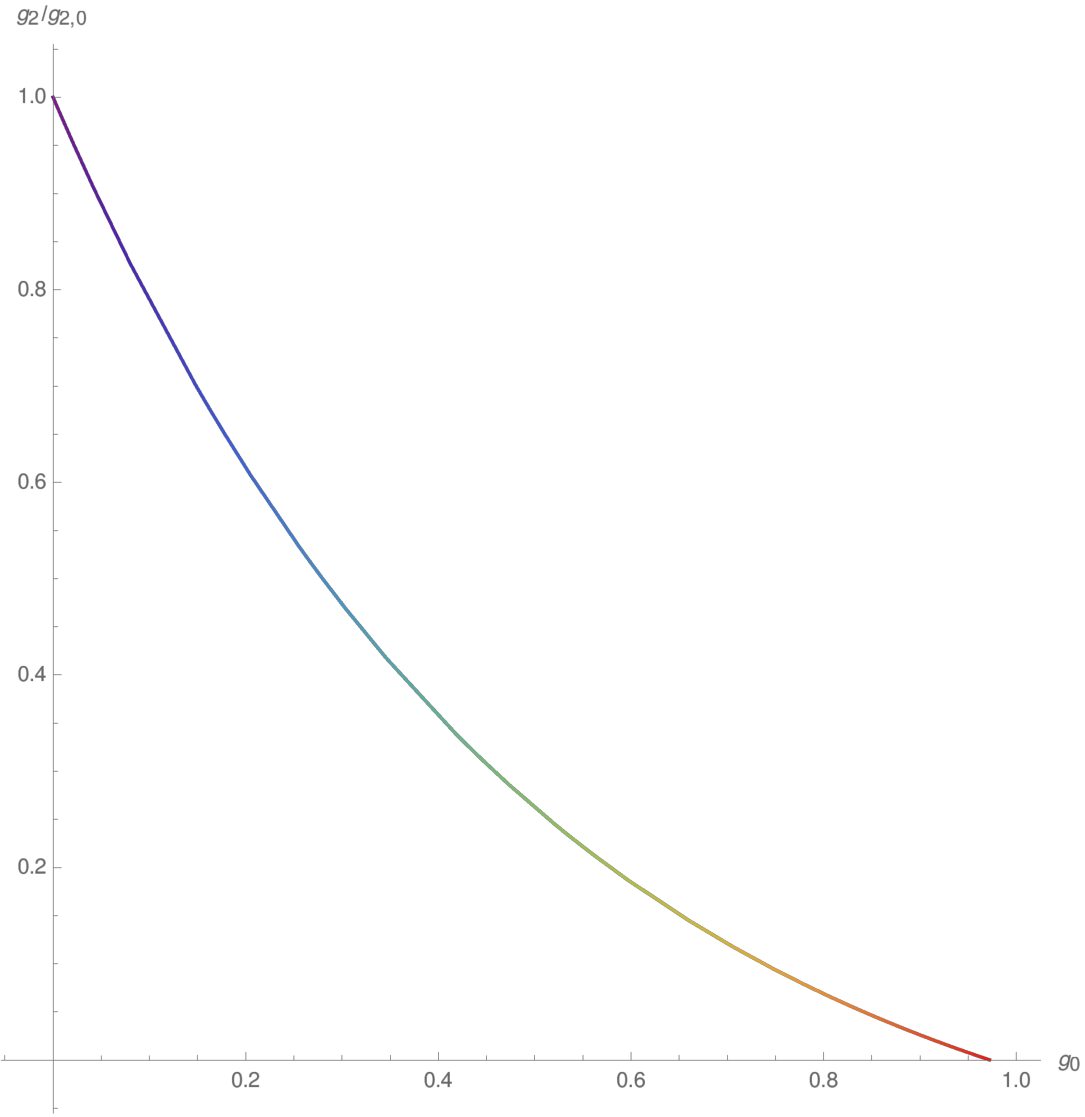
\includegraphics[scale=0.5]{4_3_1_2}
\caption{Evolving these expressions we find the following flow which reaches $g_n = 0$ for $n > 0$ fixed point. Shown is the range $t \in [0, 3]$}
\end{center}
\end{figure}

\subsubsection{Problem 3.}

For initial conditions $g_2(0) = A$ we find,
\[ g_2(t) = \frac{A}{e^{2 t} + 2 D_0 A (e^{2 t} - 1)} \quad \text{and} \quad g_0(t) = \tfrac{1}{2} \log{[(1 + 2 D_0 A) e^{2 t} - 2 D_0 A]} - t \]
Now we perform a series expansion of $Z$ using Wick's theorem, as before. We find,
\begin{align*}
Z & = \frac{1}{\sqrt{2 \pi D_0}} \int \d{\phi} e^{-\frac{\phi^2}{2 D_0} - I_t(\phi)} = \frac{1}{\sqrt{2 \pi D_0}} \int \d{\phi} e^{-\frac{\phi^2}{2 D_0} - g_0(t) - g_2(t) \phi^2}
\\
& = \frac{1}{\sqrt{2 \pi D_0}} e^{- g_0(t)} \int \d{\phi} e^{-\frac{\phi^2}{2 D_0}} \sum_{n = 0}^\infty \frac{1}{n!} g_2(t)^n \phi^{2n} 
=  e^{- g_0(t)} \sum_{n = 0}^\infty \frac{1}{n!} g_2(t)^n \frac{1}{\sqrt{2 \pi D_0}} \int \d{\phi} e^{-\frac{\phi^2}{2 D_0}}  \phi^{2n} 
\\
& = e^{- g_0(t)} \sum_{n = 0}^\infty \frac{1}{n!} g_2(t)^n \EV{\phi^{2n}}
\end{align*}
As before, by Wick's theorem, 
\[ \EV{\phi^{2n}} = (2n - 1)!! D_0^{2n} \]
and thus,
\[ Z = e^{- g_0(t)} \sum_{n = 0}^\infty (g_2(t) D_0)^n \frac{(2 n - 1)!!}{n!} \]
Apply the ratio test to the series,
\[ a_n =  (g_2(t) D_0)^n \frac{(2 n - 1)!!}{n!} \]
to find that,
\begin{align*}
L = \lim_{n \to \infty} \frac{a_{n+1}}{a_n} = g_2(t) D_0 \lim_{n \to \infty}  \frac{2 n + 1}{(n + 1)} = g_2(t) D_0 \lim_{n \to \infty} \frac{2 + 1/n}{1 + 1/n} = 2 g_2(t) D_0
\end{align*}
Therefore, the series converges when,
\[ g_2(t) < \frac{1}{2D_0} \]
For $D_0 = 1$ and $A = 3$ this occurs at,
\[ 
t_* = \tfrac{1}{2} \log{\tfrac{12}{7}} \approx 0.27 \]
For general $A$ we need to solve,
\[ g_2(t) = \frac{A}{e^{2t_*} + 2 D_0 A (e^{2 t_*} - 1)} = \frac{1}{2D_0} \]
In the limit $A \to \infty$ this reduces to,
\[ \frac{1}{2 D_0(e^{2 t_*} - 1)} = \frac{1}{2 D_0} \]
and therefore,
\[ t_* = \tfrac{1}{2} \log{2} \] 

\subsubsection{Problem 4.}

At the initial point of the flow we have $g_2(0) = A$ and all other $g_n(0) = 0$. Thus, we can calculate the following expression exactly,
\[ Z = \frac{1}{\sqrt{2 \pi D_0}} \int \d{\phi} e^{- \frac{\phi^2}{2 D_0} - I_0(\phi) } = \frac{1}{\sqrt{2 \pi D_0}} \int \d{\phi} e^{- \frac{\phi^2}{2 D_0} - A \phi^2 } = \sqrt{\frac{\pi}{2 \pi (\tfrac{1}{2} D_0^{-1} + A)}} = \frac{1}{\sqrt{1 + 2 D_0 A}} \]
In the $t \to \infty$ limit, we have shown that $g_n(t) \to 0$ for all couplings expect $g_0$ for which,
\[ \lim_{t \to \infty} g_0(t) = \lim_{t \to \infty} \left[ \tfrac{1}{2} \log{[(1 + 2 D_0 A)e^{2t} - 2 D_0 A] } - t \right] = \tfrac{1}{2} \log{(1 + 2 D_0 A)} \] 
Therefore, in the $t \to \infty$ limit of the flow we have,
\[ e^{-I_t(\phi)} = e^{-g_0(t)} = \frac{1}{\sqrt{1 + 2 D_0 A}} \]
which agrees with the initial value of $Z$. 

\subsection{QFT}

\subsubsection{Problem.}

We want to consider the Wilsonian RG flow equations for a QFT in $d$-dimensions. At some renormalization scale $\Lambda$ we can express the action as a sum of local operators in the form,
\[ I_{\Lambda}[\phi] = \sum_{I} c_I(\Lambda) \int_x \mathcal{O}_I(x) = \sum_I g_I(\Lambda) \Lambda^{\bar{\Delta}_I} \int_x \mathcal{O}_I(x) \]
where $\Delta_I$ is the dimension of $\mathcal{O}_I$ and $\bar{\Delta}_I = d - \Delta_I$.  We use the notation,
\[ q \cdot \partial_q G_n(q_1, \dots, q_n) = \sum_{i = 1}^n q_i^\mu \partial_{q_i^\mu} G_n(q_1, \dots, q_n) \]
and we have defined the dimensionless interactions in Fourier space,
\[ I_n(p) = \Lambda^{d - n} G_n(p / \Lambda) \]
Finally, we take the dimensionless propagator $\dot{D}_1(q) = \Lambda^{d - 2} \dot{D}(\Lambda q)$.
Now we apply the RG condition,
\[ \dot{I} = \tfrac{1}{2} \dot{D} \left( (\partial_\phi I)^2 - \partial^2_\phi I \right) \]
where,
\[ \dot{D} (\partial_\phi I)^2 = \int_k \dot{D}(k) \frac{\delta I}{\delta \phi(-k)} \frac{\delta I}{\delta \phi(k)} \quad \quad \dot{D} \partial^2_\phi I = \int_k \dot{D}(k) \frac{\delta}{\delta \phi(-k)} \frac{\delta}{\delta \phi(k)} I \]
When expanded order-by-order, this gives, schematically, the RG flow equations,
\begin{align*}
\dot{I}_0 & = \int \dot{D} I_2
\\
\dot{I}_2 & = I_2 \dot{D} I_2 - \int \dot{D} I_4
\\
\dot{I}_4 & = I_2 \dot{D} I_4 - \int \dot{D} I_6
\\
\dot{I}_6 & = I_2 \dot{D} I_6 + I_4 \dot{D} I_4 - \int \dot{D} I_8
\end{align*}
We will plug out dimensionless defined quantities into these flow equations. First, consider the left hand side,
\begin{align*}
\dot{I}_n(p) = \partial_t (\Lambda^{d - n} G_n(q)) = - \Lambda \partial_{\Lambda} (\Lambda^{d - n} G_n(q)) = (n  - d) \Lambda^{d - n} G_n(q) - \Lambda^{d - n + 1} \partial_\Lambda G_n(q) 
\end{align*}
where $p = \Lambda q$. By the chain rule,
\begin{align*}
- \Lambda \partial_{\Lambda} G_n(q) & = \dot{G}_n(q) - \Lambda \partial_{\Lambda} \sum_{i = 1}^n \left( \frac{p_i^\mu}{\Lambda} \right) \partial_{q_i^\mu} G_n(q) = \dot{G}_n(q) + \sum_{i = 1}^n \left( \frac{p_i^\mu}{\Lambda} \right) \partial_{q_i^\mu} G_n(q)
\\
& = \dot{G}_n(q) + \sum_{i = 1}^n q_i^\mu \partial_{q_i^\mu} G_n(q) = \dot{G}_n(q) + q \cdot \partial_q G_n(q)
\end{align*}
Putting this together,
\begin{align*}
\dot{I}_n(p) = \Lambda^{d - n} \left[ (n - d) G_n(q) + \dot{G}_n(q) + q \cdot \partial_q G_n(q) \right]
\end{align*}
Now we need to compute the right hand side. First, the ``tree-level'' term,
\begin{align*}
I_n(p) \dot{D}(p) I_m(p) = \Lambda^{d - n - m + 2}G_n(q) \dot{D}_1(q) G_n(q)
\end{align*}
and the ``loop'' term,
\begin{align*}
\int \frac{\dn{d}{k}}{(2 \pi)^d} \dot{D}(k) I_n(k) = \Lambda^{- n + 2} \int \frac{\dn{d}{k}}{(2 \pi)^d}\dot{D}_1(q) G_n(q) = \Lambda^{d - n + 2} \int \frac{\dn{d}{q}}{(2 \pi)^d} \dot{D}_1(q) G_n(q)
\end{align*}
Therefore, plugging into the schematic,
\begin{align*}
\dot{I}_n(p) = \sum_{i + j = n + 2} I_i(p) \dot{D}(p) I_j(p) - \int \dot{D} I_{n + 2}
\end{align*}
we get,
\begin{align*}
\Lambda^{d - n} [\dot{G}_n(q) + (n - d) G_n(q) + q \cdot \partial_q G_n(q)] = \Lambda^{d - n} \sum_{i + j = n + 2} G_i \dot{D}_1 G_j - \Lambda^{d - n} \int \dot{D}_1 G_{n+2}
\end{align*}
which implies that,
\begin{align*}
\dot{G}_n(q) = [(d - n) - q \cdot \partial_q] G_n(q) + \sum_{i + j = n + 2} G_i \dot{D}_1 G_j - \int \dot{D}_1 G_{n+2}
\end{align*}
or, in expanded schematic form,
\begin{align*}
\dot{G}_0 & = d G_0 + \int \dot{D}_1 G_2
\\
\dot{G}_2 & = [(d - 2) - q \cdot \partial_q] G_2 + G_2 \dot{D}_1 G_2 - \int \dot{D}_1 G_4
\\
\dot{G}_4 & = [(d - 4) - q \cdot \partial_q] G_4 + G_2 \dot{D}_1 G_4 - \int \dot{D}_1 G_6
\\
\dot{G}_6 & = [(d - 6) - q \cdot \partial_q] G_6 + G_2 \dot{D}_1 G_6 + G_4 \dot{D}_1 G_4 - \int \dot{D}_1 G_8
\end{align*}
\section{Asymptotic Behavior of Wilsonian RG Flow at Weak Coupling}

\subsection{Existence and Properties of Solutions}

\subsection{Friction terms, large logs and beta functions: a toy model}

Consider the phase space motion of a particle in 1D with a Hamiltonian,
\[ H = \epsilon (\tfrac{1}{2} P^2 + V(Q)) \]
with an additional friction term $F = - \gamma P$. We scale time such that $\gamma = 1$. Then the system has equations of motion,
\[ \dot{Q} = \epsilon P \quad \quad \dot{P} = - P - \epsilon V'(Q) \]

\subsubsection{Problem 1.}

Consider the case $V(Q) = Q^2$. We will expand the motion in an $\epsilon$-expansion,
\[ Q = Q_0 + \epsilon Q_1 + \epsilon^2 Q_2 + \cdots \quad \quad P = P_0 + \epsilon P_1 + \epsilon^2 P_2 \]
At first order, the equations of motion give,
\[ \dot{Q}_0 = 0 \quad \quad \dot{P}_0 = - P_0 \]
and thus for initial conditions $(Q, P) = (q_0, p_p)$ we get,
\[ Q_0 = q_0 \quad \quad P_0(t) = p_0 e^{-t} \]
At first-order, the equations of motion are,
\[ \dot{Q}_1 = P_0 \quad \quad \dot{P}_1 = - P_1 - V'(q_0) \]
which, assuming that we set higher-order solutions to zero in the initial conditions, is solved by,
\[ Q_1(t) = (1 - e^{-1}) p_0 \quad \quad P_1(t) = (-1 + e^{-t}) V'(q_0) \]
Finally, expanding the equations of motion to third-order gives,
\[Q_2 = P_1 \quad \quad \dot{P}_2 = - P_2 - V''(q_0) Q_1 \]
which, using the above solutions and zero initial conditions, are solved by,
\[ Q_1(t) = (1 - t - e^{-1}) V'(q_0) \quad \quad P_2(t) = (-1 + (t + 1)e^{-t})) p_0 V''(q_0) \]
By continuing in this way we can solve for the $\beta$-function explicitly by rewriting these equations in terms of $Q$. However, it is simpler to start from the assumption that these is some functional dependence, $P = P(Q)$. Then,
\[ \beta(Q) = - \dot{Q} = - \epsilon P(Q) \]
Using the second equation of motion,
\[ \dot{P} = P'(Q) \dot{Q} = - P - \epsilon V'(Q) \] 
Therefore,
\[ P(Q) = - \epsilon V'(Q) - \epsilon P'(Q) P(Q) \]
We will solve this functional equation via an expansion in $\epsilon$. For $V(Q) = Q^2$ we have the equation,
\[ P(Q) = - \epsilon \left( 2 Q + P'(Q) P(Q) \right) \]
At first-order in $\epsilon$ we have,
\[ P(Q) = -2 \epsilon Q \]
at second-order,
\[ P(Q) = -\epsilon (2 Q + (-2 \epsilon)(-2\epsilon Q)) = - \epsilon(2 + 4 \epsilon^2) Q \]
Notice that, at each stage, $P(Q) \propto -\epsilon Q$. Therefore, we suppose there exists a solution of the form,
\[ P(Q) = - \epsilon N(\epsilon) Q \]
Plugging in,
\[ -\epsilon N(\epsilon) Q = -\epsilon (2 Q + (-\epsilon N(\epsilon))^2 Q) = - \epsilon(2 + \epsilon^2 N(\epsilon)^2) Q \]
Therefore we find,
\[ N(\epsilon) = 2 + \epsilon^2 N(\epsilon)^2 \]
This implies that,
\[ N(\epsilon) = \frac{1 \pm \sqrt{1 - 8 \epsilon^2}}{2 \epsilon^2} \]
Therefore, the beta function, is,
\[ \beta(Q) = \epsilon^2 N(\epsilon) Q \] 
However, in this case we can easily solve the exact differential equation,
\[ \dot{Q} = \epsilon P \quad \quad \dot{P} = - P - 2 \epsilon Q \]
by differentiating the first,
\[ \ddot{Q} = \epsilon \dot{P} = - \epsilon P - 2 \epsilon^2 Q \]
This has the form,
\[ \ddot{Q} + \dot{Q} + 2 \epsilon^2 Q = 0 \]
of a damped harmonic oscillator in the over-damped regime. We look for exponential solutions of the form,
\[ Q(t) = Q_0 e^{-\alpha t} \]
where $\alpha \in \C$. Plugging in, we find the characteristic polynomial,
\[ \alpha^2 - \alpha + 2 \epsilon^2 = 0 \]
which has solutions,
\[ \alpha(\epsilon) = \frac{1 \pm \sqrt{1 - 8 \epsilon^2}}{2} \]
that look suspiciously familiar. In fact, 
\[ \beta(Q) = \epsilon^2 N(\epsilon) Q = \alpha(\epsilon) Q \]
which exactly expresses the fact that,
\[ \dot{Q} = - \beta(Q) = - \alpha(\epsilon) Q \]
the defining property of such exponential solutions. A general solution to the differential equations can therefore be written as a sum of these exponential modes,
\begin{align*}
Q(t) & = A_{+} e^{-\alpha_{+}(\epsilon) t} + A_{-} e^{-\alpha_{-}(\epsilon) t} = A_{-} e^{- \alpha_{-}(\epsilon) t} \left( 1 + \frac{A_{+}}{A_{-}} e^{- (\alpha_{+}(\epsilon) - \alpha_{-}(\epsilon)) t} \right)
\\
& = A_{-} e^{- \alpha_{-}(\epsilon) t} \left( 1 + \frac{A_{+}}{A_{-}} e^{- \sqrt{1 - 8 \epsilon^2} \: t} \right)
\end{align*}
This shows that all solutions are attracted to the $\alpha_{-}(\epsilon)$ mode which is a 1D subspace of solutions characterized by the flow equation,
\[ \beta(Q) = \epsilon^2 N_{-}(\epsilon) Q = \frac{1 - \sqrt{1 - 8 \epsilon^2}}{2} Q \]
The difference of an arbitrary solution from this subspace decays exponentially with a rate constant $\sqrt{1 - 8 \epsilon^2}$. Therefore, the other solution for $\beta(Q)$ corresponds to a IR-repulsive unstable fixed-flow surface. 

\subsubsection{Problem 2.}

Let $t_*$ be a finite reference time as we take $t_0 \to - \infty$ in the high UV limit. We will express quantities in terms of the renormalized value $q_*$ at $t_*$. From the given formula to second-order with the irrelevant term $p_0 = 0$ we find, 
\[ q_* = Q(t_*) = q_0 - \epsilon^2(t_* - t_0 - 1)V'(q_0) + O(\epsilon^3) \] 
We must hold this finite as the ``bare'' terms $q_0$ and $t_0$ diverge. Now consider,
\[ Q(t) = q_0 - \epsilon^2 (t - t_0 - 1) V'(q_0) + (\epsilon^3) \]
and thus,
\[ Q(t) - q_* = -\epsilon^2(t - t_*) V'(q_0) + O(\epsilon^3) \]
Using the equation,
\[ P(t) = - \epsilon V'(q_0) + O(\epsilon^2) \]
we find,
\[ Q(t) = q_* + \epsilon (t - t_*) P(t) + O(\epsilon^3) \]
However, for $P(t)$ and equivalently $Q(t)$ to be finite we need $V'(q_0)$ to be finite up to this order of perturbation theory. Consider,
\[ V'(q_*) = V'(q_0 - \epsilon^2(t_* - t_0 - 1) V'(q_0)) = V'(q_0) - \epsilon^2(t_* - t_0 - 1) V'(q_0) V''(q_0)  = V'(q_0) + O(\epsilon^2) \]
Therefore,
\[ P(t) = - \epsilon V'(q_*) + O(\epsilon^2) \]
and furthermore, 
\[ Q(t) = q_* - \epsilon^2 (t - t_*) V'(q_*) + O(\epsilon) \] 
are both finite at this order of perturbation theory. Thus all observables expressed in terms of the renormalized variables $t_*$ and $q_*$ are finite. The renormalizablity of this model is simply a consequence of the fact that fixing $t_*$ and $q_*$ we can integrate the equations of motion back in time to $t_0$ and $q_0$ arbitrarily far to $t_0 \to - \infty$. The solution expressed in terms of this initial point $t_0$, $q_0$ is exactly the same solution since, by construction, it matches the solution with initial point $t_*$, $q_*$ and thus such a solution must be finite when Written in terms of the initial point $t_0$, $q_0$.  


\subsubsection{Problem 3.}

Now we consider the potential $V(Q) = \tfrac{1}{4} \alpha Q^4$ with anti-friction. The equations of motion are,
\[ \dot{Q} = \epsilon P \quad \quad \dot{P} = P - \epsilon \alpha Q^3 \]
If we reverse $t \mapsto - t$ and $P \mapsto - P$ then we recover,
\[ \dot{Q} = \epsilon P \quad \quad \dot{P} = - P - \epsilon \alpha Q^3 \]
which is exactly the equations of motion we have been considering. Since we have reversed time, rather than an IR repulsive point we need to find a IR attractive point since our IR is the original UV and such a point is a UV fixed point. We showed that, to first-order in $\epsilon$, the $\beta$-function for $Q$ is given by,
\[ \beta(Q) = - \epsilon P(Q) = \epsilon^2 V'(Q) = \epsilon^2 \alpha Q^3 \] 
Therefore, the theory has a fixed point flow of $P = - \epsilon \alpha Q^3$. Therefore, if we take,
\[ P(0) = + \epsilon \alpha Q(0)^3 \]
in the original non-time-reversed theory we should have an IR repulsive fixed point away from which all trajectories grow exponentially. We will now verify that trajectories with these initial conditions in the anti-friction theory are fine-tuned to not have exponentially growing modes in the IR. Let $Q(0) = q_0$ and then $p_0 = \epsilon \alpha q_0^3$. We have the equations of motion,
\[ \dot{Q} = \epsilon P \quad \quad \dot{P} = P - \epsilon \alpha Q^3 \] 
We solve these equations with an $\epsilon$-expansion,
\[ Q(t) = Q_0 + \epsilon Q_1 + \epsilon^2 Q_2 + \cdots \quad \quad P(t) = P_0 + \epsilon P_1 + \epsilon^2 P_2 + \cdots \]
Thus, we find to zeroth-order,
\[ Q_0 = q_0 \quad \quad P_0 = 0 \]
At first-order, 
\[ \dot{Q}_1 = P_0 = 0 \quad \quad \dot{P}_1 = P_1 - \alpha Q_0^3 = P_1 - \alpha q_0^3 \]
But $P_1(0) = \alpha q_0^3$ and thus we have,
\[ Q_1 = 0 \quad \quad P_1 = \alpha q_0^3 \]
At second order,
\[ \dot{Q}_2 = P_1 = \alpha q_0^3 \quad \quad \dot{P}_2 = P_2 - 3 \alpha Q_0^2 Q_1 = P_2 \]
and therefore, $Q_2$ grows linearly and $P_2$ exponentially except that $P_2(0) = 0$ and thus we have $P_2 = 0$. Together we have, 
\[ Q(t) = Q_0 + \epsilon^2 \alpha q_0^3 (t - t_0) + O(\epsilon^3) \quad \quad P(t) = \epsilon \alpha q_0^3 + O(\epsilon^3) \]
so there is no exponential growth at least up to order $\epsilon$. 

\subsection{Back to QFT: the stable subspace, renormalizablity and the beta function}

\section{Additional Work: The RG Flows of Related Theories}

Here we will investigate how the RG flows quantitatively evolve for a few concrete $d = 3 + 1$ dimensional reasonable QFTs. These will be, a two-particle scalar Yukawa theory, a fermion-scalar meson true Yukawa theory, and a fermion with quartic self-interactions which is the effective field theory of the above Yukawa theory in the limit of a heavy meson. These theories were carefully chosen to focus on a relevant, marginal, and irrelevant coupling respectively. We will perform full renormalized perturbation theory at the one-loop level to find the vertex corrections for each of these theories and determine the sorts of RG flows that appear. 

\subsection{Scalar Yukawa Theory}

We first return to our old friend the Scalar Yukawa theory with a Lagrangian density, 
\[ \lagrange = \lagrange_0 + \lagrange_{\ipic} + \lagrange_{\text{ct}} \quad \quad \lagrange_0 = \tfrac{1}{2} \partial_\mu \phi \partial^\mu \phi - \tfrac{1}{2} M^2 \phi^2 + \partial_\mu \dpsi \partial^\mu \psi - m^2 \dpsi \psi \quad \quad \lagrange_{\ipic} = -g \dpsi \psi \meson \] 
with field strength renormalization giving a counter term of each type in the Lagrangian. Luckily, we have already computed the vertex function of this theory on that monster of a problem set last year. However, I will reproduce the computation here for completeness.

\subsubsection{Vertex Renormalization}

The shift between the physical and bare coupling constants and the field strength renormalization factors introduce
a new vertex,
\begin{equation*}
\begin{tikzpicture}[baseline = -0.1cm]
\begin{feynman}
\vertex [crossed dot] (a) {};
\vertex [below left=of a] (b);
\vertex [above left=of a] (c);
\vertex [right=of a] (d);
\diagram* {
(a) -- [fermion] (b),
(c) -- [fermion] (a),
(a) -- [scalar] (d)
};
\end{feynman}
\end{tikzpicture}
= - i c_4
\end{equation*} 
At the one loop level, there are only three diagrams which contribute to the vertex function,
\begin{equation*}
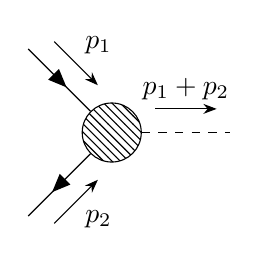
\begin{tikzpicture}[baseline = (b)]
\begin{feynman}
\vertex [blob] (b) {};
\vertex [above left=of b] (a);
\vertex [below left=of b] (c);
\vertex [right=of b] (d);
\diagram* {
(a) -- [fermion, momentum = $p_1$] (b) -- [fermion, rmomentum = $p_2$] (c),
(b) -- [scalar, momentum=$p_1 + p_2$] (d)
};
\end{feynman}
\end{tikzpicture}
 = - i \Gamma(p_1, p_2)
\end{equation*}

\begin{equation*}
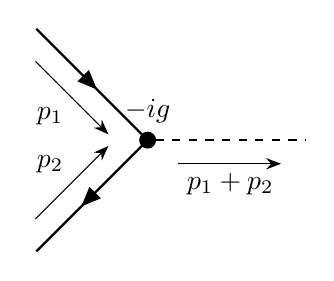
\begin{tikzpicture}[baseline = (a)]
\begin{feynman}[large]
\vertex [dot, label = $-ig$] (a) {};
\vertex [below left=of a] (b);
\vertex [above left=of a] (c);
\vertex [right=of a] (d);
\diagram* {
(a) -- [fermion, rmomentum'=$p_2$] (b),
(c) -- [fermion, momentum'=$p_1$] (a),
(a) -- [scalar, momentum'=$p_1 + p_2$] (d)
};
\end{feynman}
\end{tikzpicture}
\quad
\mathlarger{+}
\quad 	
\feynmandiagram [horizontal = a to b, baseline = (a)] {
	i1 -- [fermion, momentum'=$p_1$] t1 -- [fermion, momentum=$p_1 - k$] a,
	a -- [fermion, rmomentum=$p_2 + k$] t2 -- [fermion, rmomentum'=$p_2$] i2, 
	t1 -- [scalar, momentum'=$k$] t2,
	a -- [scalar, momentum'=$p_1 + p_2$ ] b
	};
\quad
\mathlarger{+}
\quad 	
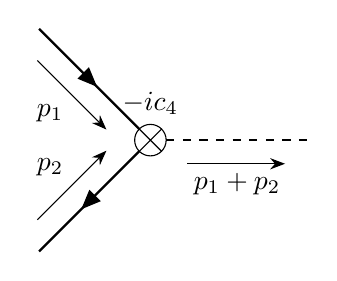
\begin{tikzpicture}[baseline = (a)]
\begin{feynman}[large]
\vertex [crossed dot, label = $-ic_4$] (a) {};
\vertex [below left=of a] (b);
\vertex [above left=of a] (c);
\vertex [right=of a] (d);
\diagram* {
(a) -- [fermion, rmomentum'=$p_2$] (b),
(c) -- [fermion, momentum'=$p_1$] (a),
(a) -- [scalar, momentum'=$p_1 + p_2$] (d)
};
\end{feynman}
\end{tikzpicture}
\end{equation*}
Using the Feynman rules,
\[ - i \Gamma(p_1, p_2) = (-ig) + (-ig)^3 \int \frac{\mathrm{d}^4 k}{(2 \pi)^4} \frac{i}{k^2 - M^2 + i \epsilon} \cdot \frac{i}{(p_1 - k)^2 - m^2 + i \epsilon} \cdot \frac{i}{(p_2 + k)^2 - m^2 + i \epsilon} - i c_4	\]
Therefore, we better evaluate this integral, 
\begin{align*}
V(p_1, p_2) =  \int \frac{\mathrm{d}^4 k}{(2 \pi)^4} \frac{i}{k^2 - M^2 + i \epsilon} \cdot \frac{i}{(p_1 - k)^2 - m^2 + i \epsilon} \cdot \frac{i}{(p_2 + k)^2 - m^2 + i \epsilon}
\end{align*}
Introducing Feynman parameters and remembering the factor of $(n-1)!$,
\begin{align*}
V(p_1, p_2) & = -2i \int \frac{\mathrm{d}^4 k}{(2 \pi)^4} \int_0^1 \frac{\d{x} \d{y} \d{z} \delta(x + y + z - 1)}{[x k^2 + y (p_1 - k)^2 + z (p_2 + k)^2 - x M^2 - (y + z) m^2 + i \epsilon]^3}
\\
& = -2i \int \frac{\mathrm{d}^4 k}{(2 \pi)^4} \int_0^1 \frac{\d{x} \d{y} \d{z} \delta(x + y + z - 1)}{[k^2 - 2 y p_1 \cdot k + y p_1^2 + 2 z p_2 \cdot k + z p_2^2 - x M^2 - (y + z) m^2 + i \epsilon]^3}
\\
& = -2i \int \frac{\mathrm{d}^4 k}{(2 \pi)^4} \int_0^1 \frac{\d{x} \d{y} \d{z} \delta(x + y + z - 1)}{[(k - yp_1 + z p_2)^2 - (y p_1 - z p_2)^2 + y p_1^2 + z p_2^2 - x M^2 - (y + z) m^2 + i \epsilon]^3}
\\
& = -2i \int \frac{\mathrm{d}^4 \ell}{(2 \pi)^4} \int_0^1 \frac{\d{x} \d{y} \d{z} \delta(x + y + z - 1)}{[\ell^2 - (y p_1 - z p_2)^2 + y p_1^2 + z p_2^2 - x M^2 - (y + z) m^2 + i \epsilon]^3}
\end{align*}
Now it is time to set $\Delta = (y p_1 - z p_2)^2 - y p_1^2 - z p_2^2 + x M^2 + (y + z) m^2 - i \epsilon$ and perform a Wick rotation $\ell^0 = i \ell_E^0$ so the integral becomes,
\begin{align*}
V(p_1, p_2) & = -2 \int \frac{\mathrm{d}^4 \ell_E}{(2 \pi)^4} \int_0^1 \frac{\d{x} \d{y} \d{z} \delta(x + y + z - 1)}{[\ell_E^2 + \Delta]^3}
\\
& = - \frac{4 \pi^2}{(2 \pi)^4} \int_0^1 \d{x} \d{y} \d{z} \delta(x + y + z - 1) \int_{0}^\infty \d{\ell_E} \frac{\ell_E^3}{[\ell_E^2 + \Delta]^3}
\end{align*}
However, 
\[ - \deriv{}{x} \frac{2 x^2 + \Delta}{4(x^2 + \Delta)^2} = -\frac{x}{(x^2 + \Delta)^2} + \frac{(2 x^2 + \Delta)x}{(x^2 + \Delta)^3} = \frac{x^3}{(x^2 + \Delta)^3}\]
Therefore, 
\[ \int_{0}^\infty \d{\ell_E} \frac{\ell_E^3}{[\ell_E^2 + \Delta]^3} = \left[ -\frac{2 x^2 + \Delta}{4(x^2 + \Delta)^2} \right]_{0}^\infty = \frac{1}{4 \Delta} \]
so the integral $V(p_1, p_2)$ is actually finite. At last,
\[ V(p_1, p_2) = -\frac{1}{16 \pi^2} \int_0^1 \frac{\d{x} \d{y} \d{z} \delta(x + y + z - 1) }{(y p_1 - z p_2)^2 - y p_1^2 - z p_2^2 + x M^2 + (y + z) m^2 - i \epsilon} \]
Therefore, the vertex function becomes,
\[ - i \Gamma(p_1, p_2) = (-ig) - \frac{ig^3}{16 \pi^2} \int_0^1 \frac{\d{x} \d{y} \d{z} \delta(x + y + z - 1) }{(y p_1 - z p_2)^2 - y p_1^2 - z p_2^2 + x M^2 + (y + z) m^2 - i \epsilon} - i c_4\]

\subsubsection{A First Attempt at the $\beta$-Function}

Define the coupling at scale $\mu$ by space-like (unphysical) momenta $p_1 = p_2 = (0, \mu, 0, 0)$ in line with the RG conventions of Peskin and Schroeder Chapter 12. This gives,
\[  g(\mu) = \Gamma(\mu) \]
where,
\begin{align*}
 - i \Gamma(\mu) = (-ig) - \frac{ig^3}{16 \pi^2} \int_0^1 \frac{\d{x} \d{y} \d{z} \delta(x + y + z - 1) }{(\mu^2 + m^2) (y + z) - \mu^2(y - z)^2 + x M^2} - i c_4
\end{align*}
If we choose to renormalize at some scale $g = g(\mu)$ then we find the expressions,
\begin{align*}
g(e^{-t} \mu)&  - g(\mu) = \Gamma(e^t \mu) - \Gamma(\mu)
\\
& = \frac{g(\mu)^3}{16 \pi^2} \int_0^1  \left[ \frac{\d{x} \d{y} \d{z} \delta(x + y + z - 1) }{(e^{-2t} \mu^2 + m^2) (y + z) - e^{-2t} \mu^2(y - z)^2 + x M^2} -
\frac{\d{x} \d{y} \d{z} \delta(x + y + z - 1) }{(\mu^2 + m^2) (y + z) - \mu^2(y - z)^2 + x M^2}  \right]
\end{align*}
Thus,
\begin{align*}
\dot{g} = \frac{g(\mu)^3}{8 \pi^2} \int_0^1 \d{x} \d{y} \d{z} \delta(x + y + z - 1) \frac{\mu^2(y + z) - \mu^2 (y - z)^2}{[(\mu^2 + m^2) (y + z) - \mu^2(y - z)^2 + x M^2]^2}
\end{align*}
This is easily computed in the limit $\mu \gg m, M$ i.e. if the effectively massless case. Then, the integral becomes, 
\begin{align*}
\dot{g}(\mu) = \frac{g(\mu)^3}{8 \pi^2 \mu^2} \int_0^1  \frac{\d{x} \d{y} \d{z} \delta(x + y + z - 1)}{(y + z) - (y - z)^2} = \frac{g(\mu)^3}{8 \pi^2 \mu^2} \log{4}
\end{align*}
This does not have the standard form of a $\beta$-function that we might naively expect since it is $\mu$ dependent. However this is not at all surprising because $g$ is not a dimensionless coupling it has mass dimension one. Therefore, we should consider the dimensionless coupling,
\[ g(\mu) = \mu \tilde{g}(\mu) \] 
Then we find,
\[ \deriv{}{t} g(e^{-t} \mu) = - \mu \tilde{g} + \mu \dot{\tilde{g}} \]
which implies that,
\[ \dot{\tilde{g}}(\mu) = \tilde{g}(\mu) + \mu^{-1} \dot{g}(\mu) = \tilde{g}(\mu) + \frac{g(\mu)^3}{8 \pi^2 \mu^3} \log{4} = \tilde{g} + \frac{\tilde{g}(\mu)^3}{8 \pi^2} \log{4} \]
Therefore, the analog of the $\beta$-function is,
\[ 
\deriv{\tilde{g}(\mu)}{\log{\mu}} = \beta(\tilde{g}(\mu)) \quad \quad \beta(\tilde{g}) = - \tilde{g} - \frac{\log{4}}{8 \pi^2} \tilde{g}^3 
\] 
The first term gives the classical scaling predicted by the Wilsonian RG. 

\subsubsection{An Issue Arises}

But wait! We have been to hasty. If we renormalize at the point $p^2 = - \mu^2$ and then compute $\Gamma(e^{-t} \mu)$ we are not actually computing the correct amplitudes in the new renormalized theory. This is because part of the renormalization conditions are to fix the propagator pole and residue by imposing the conditions,
\[ \Sigma(p^2 = - \mu^2) = 0 \quad \quad \deriv{\Sigma(p^2)}{p^2} \bigg|_{p^2 = - \mu^2} = 0 \]
on the sum of 1PI diagrams. However, at the new scale, $\Sigma$ may have a nonzero derivative so we are not working in a properly renormalized theory. The issue is better seen by considering the field strength renormalization. Because we are imposing conditions at the renormalization point $p^2 = - \mu^2$ away from the physical mass pole, the field strength renormalization factor $Z$ we introduce does not cancel the field strength factor in the K\"{a}llén–Lehmann spectral representation and therefore will show up in amplitudes via the LSZ reduction formula. We have fixed,
\[ \bra{\Omega} \phi(p) \phi(-p) \ket{\Omega} = \frac{i}{p^2 - m^2 + i \epsilon} \]
at the point $p^2 = - \mu^2$. However, we know that the bare fields satisfy,
\[ \bra{\Omega} \phi_0(p) \phi_0(-p) \ket{\Omega} \sim \frac{i Z_{\text{phys}}}{p^2 - m^2 + i \epsilon} \] 
and thus,
\[ \bra{\Omega} \phi(p) \phi(-p) \ket{\Omega} = Z^{-1}  \bra{\Omega} \phi_0(p) \phi_0(-p) \ket{\Omega} \sim \frac{i Z^{-1} Z_{\text{phys}}}{p^2 - m^2 + i \epsilon} \]
this means that the effective field strength which appears in the LSZ reduction formula for the renormalized fields is,
\[ Z^{\text{eff}} = Z^{-1} Z_{\text{phys}} \]  
Since the factor $Z$ is $\mu$ dependent since it is determined by a renormalization condition at $Z$ we will find additional $\mu$ dependence in the $\beta$-function. The correct renormalized parameters work as follows,
\[ Z^{\text{eff}}_{\psi}(e^{-t} \mu) (Z^{\text{eff}}_{\phi}(e^{-t} \mu))^{1/2} g(e^{-t} \mu) = Z^{\text{eff}}_{\psi}(\mu) (Z^{\text{eff}}_{\phi})^{1/2}(\mu) \Gamma(e^{-t} \mu ; \mu) \]
where $\Gamma(e^{-t} \mu ; \mu)$ is the vertex function renormalized at $\mu$. By including such field strength factors, we are, in effect, computing the correlation function $G^{(3)}$ at one-loop which includes the external leg corrections which shift the field strength. Writing out the renormalized field strength factors and canceling the factors of $Z_{\text{phys}}$ in the above equation we get,
\[ g(\epsilon^{-t} \mu) = \frac{Z_{\psi}(e^{-t} \mu)Z_{\phi}(e^{-t} \mu)^{1/2}}{Z_{\psi}( \mu)Z_{\phi}(\mu)^{1/2}} \Gamma(e^{-t} \mu ; \mu) = g(\mu) - t \left[ \deriv{\Gamma}{\log{\mu}} + g(\mu) \deriv{\log{Z_{\psi}}}{\log{\mu}} + g(\mu) \frac{1}{2} \deriv{\log{Z_{\phi}}}{\log{\mu}} \right] \]
Therefore, the logarithmic derivatives of $Z$ with respect to $\mu$ will also enter the correct expression for change in coupling with renormalization scale. Therefore we unfortunately will need to compute the field strength renormalization. Will will then apply the Callan-Symanzik equation to systematically derive the $\beta$-function. 

\subsubsection{The Dressed Propagators}

Again, we already derived the dressing of both propagators in this theory. I will not go though the derivation again but simply state the results here. 
For the $\psi$ propagator,
\[ \Sigma_\psi(p^2) = \frac{g^2}{16 \pi^2} \left[ \int_{0}^{1} \d{x} \log{\left[ x(x - 1) p^2 + x m^2 + (1 - x) M^2 \right]} \right] + c_2 + p^2 c_6 \]
which, applying the renormalization conditions above fixes the counter-terms to given the form,
\begin{align*}
\Sigma_\psi(p^2) & = \frac{g^2}{16 \pi^2} \left[ \int_{0}^{1} \d{x} \log{\left[ \frac{x(x - 1) p^2 + x m^2 + (1 - x) M^2}{x(1 - x)\mu^2 + x m^2 + (1 - x) M^2} \right]}  \right.
\\
& \left. \quad \quad \quad - (p^2 + \mu^2) \int_{0}^{1} \d{x} \frac{x(x - 1)}{x(1 - x)\mu^2 + x m^2 + (1 - x) M^2} \right]
\end{align*}
Taking the limit $\mu \gg m, M$ we find,
\[ \Sigma_\psi(p^2) = \frac{g^2}{16 \pi^2} \left[ \log{\left( \frac{p^2}{-\mu^2} \right)} + \mu^{-2} (p^2 + \mu^2) \right] \]
Therefore, 
\begin{align*}
Z_\psi(e^{-t} \mu) & = Z_{\psi}(\mu) \left(1 - \deriv{\Sigma_\psi}{p^2} \bigg|_{p^2 = - e^{-2t}\mu^2} \right)^{-1} = Z_\psi(\mu) \left( 1 + \frac{g^2}{16 \pi^2 \mu^2} \left( \frac{1}{e^{-2t} \mu^2} - \frac{1}{\mu^2} \right) \right)^{-1} 
\\
& = Z_\psi(\mu) \left( 1 + \frac{g^2}{8 \pi^2 \mu^2} t  + O(t^2) \right)^{-1} = Z_\psi(\mu) \left( 1 - \frac{g^2}{8 \pi^2 \mu^2} t  + O(t^2) \right)
\end{align*}
and therefore,
\[ \deriv{\log{Z_{\psi}}}{\log{\mu}} = \frac{g^2}{8 \pi^2 \mu^2} \]
Exactly similarly, for the $\phi$ propagator, 
\[ \Sigma_\phi(p^2) = \frac{g^2}{16 \pi^2} \left[ \gamma_E + \log{\delta} + \int_{0}^{1} \d{x} \log{\left[ x(x-1)p^2 + m^2 - i \epsilon \right]} \right] + c_3 + p^2 c_5  \]
which, applying the renormalization conditions above fixes the counter-terms to given the form,
\[ \Sigma_\phi(p^2) = \frac{g^2}{16 \pi^2} \left[ \int_{0}^{1} \d{x} \log{\left[\frac{x(x-1)p^2 + m^2 - i \epsilon}{x(1-x)\mu^2 + m^2 - i \epsilon}\right]} - (p^2 + \mu^2) \int_{0}^{1} \d{x} \frac{x(x-1)}{x(1-x)\mu^2 + m^2 - i \epsilon} \right] \]
As usual, we proceed in the massless limit,
\[ \Sigma_\phi(p^2) = \frac{g^2}{16 \pi^2} \left[ \log{\left( \frac{p^2}{-\mu^2} \right)} + \mu^{-2} (p^2 + \mu^2) \right] \]
Therefore, 
\begin{align*}
Z_\phi(e^{-t} \mu) & = Z_\phi(\mu) \left(1 - \deriv{\Sigma_\phi}{p^2} \bigg|_{p^2 = - e^{-2t}\mu^2} \right)^{-1} = Z_\phi(\mu) \left( 1 + \frac{g^2}{16 \pi^2 \mu^2} \left( \frac{1}{e^{-2t} \mu^2} - \frac{1}{\mu^2} \right) \right)^{-1} 
\\
& = Z_\phi(\mu) \left( 1 + \frac{g^2}{8 \pi^2 \mu^2} t  + O(t^2) \right)^{-1} =  Z_\phi(\mu) \left( 1 - \frac{g^2}{8 \pi^2 \mu^2} t  + O(t^2) \right)
\end{align*}
and therefore,
\[ \deriv{\log{Z_{\phi}}}{\log{\mu}} = \frac{g^2}{8 \pi^2 \mu^2} \]
These contributions are identical because the two loops become identical themselves in the limit when the different masses become irrelevant. 

\subsubsection{The RG Flow and $\beta$-Function At Last}

Now that we have computed all the necessary quantities, it is time to put these together to find the flow of coupling constants. We showed that,
\[ \dot{g} = - \left[ \deriv{\Gamma}{\log{\mu}} + g(\mu) \deriv{\log{Z_{\psi}}}{\log{\mu}} + \frac{1}{2} g(\mu) \deriv{\log{Z_{\phi}}}{\log{\mu}} \right] = - \frac{g^3}{16 \pi^2 \mu^2} (3 - 2 \log{4}) \]
and thus,
\[ \dot{\tilde{g}} = \tilde{g} - \frac{\tilde{g}^3}{16 \pi^2} (3 - 2 \log{4})  \]
Since the coefficient $3 - 2 \log{4}$ is actually positive, this additional contribution actually changes the sign of the quantum part of the $\beta$-function.
\bigskip\\
We can make a similar derivation via the Callan-Symanzik equation for the correlation function with 2 external $\psi$ lines and one external $\phi$ line. We have,
\[ \left( \pderiv{}{\log{\mu}} + \beta(\tilde{g}(\mu)) \pderiv{}{\tilde{g}} + 2 \gamma_\psi + \gamma_\phi \right) G^{\psi^2 \phi} = 0 \]  
The vertex function has the structure of amputated diagrams plus leg corrections. We already computed the amputated part which is exactly the vertex diagram. Thus, at one-loop,
\[ G^{\psi^2 \phi}(p_1, p_2) = \left[ - i \Gamma(p_1, p_2)  - i g \frac{\Sigma_{\psi}(p_1)}{p_1^2 - m^2} - i g \frac{\Sigma_{\psi}(p_2)}{p_2^2 - m^2} - i g \frac{\Sigma_{\psi}(p_3)}{p_3^2 - m^2}\right] \frac{i}{p_1^2 - m^2} \frac{i}{p_2^2 - m^2} \frac{i}{p_3^2 - m^2}  \]
where I have removed the overall momentum conserving delta function. Taking the momentum independent part of the derivative of this amplitude with respect to the renormalization scale holding the coupling constant $\tilde{g}$ fixed gives,
\[ \pderiv{}{\log{\mu}} G^{\psi^2 \phi} = -i \left(\mu \tilde{g} + \frac{g^3 \log{4}}{8 \pi^2 \mu^2} - \frac{3 g^3}{8 \pi^2 \mu^2} \right) \frac{i}{p_1^2 - m^2} \frac{i}{p_2^2 - m^2} \frac{i}{p_3^2 - m^2} \]
Furthermore, at tree-level (since it enters the Callan-Symanzik equation multiplied by higher-order quantities) we have,
\[ \pderiv{}{\tilde{g}} G^{\psi^2 \phi} = (-i \mu) \frac{i}{p_1^2 - m^2} \frac{i}{p_2^2 - m^2} \frac{i}{p_3^2 - m^2} \]
Finally, we have already computed,
\begin{align*}
\gamma_\psi = \frac{1}{2} \deriv{\log{Z_\psi}}{\log{\mu}} = \frac{g^2}{16 \pi^2 \mu^2} \quad \quad \gamma_\phi = \frac{1}{2} \deriv{\log{Z_\phi}}{\log{\mu}} = \frac{g^2}{16 \pi^2 \mu^2}
\end{align*}
Therefore\footnote{Remembering that terms like $\gamma_\phi G^{\psi^2 \phi}$ enter multiplied by the vertex function to tree-level i.e. $-ig$ to make the equation at consistent order in perturbation theory.},
\begin{align*}
- i \left( \mu \tilde{g} + \frac{g^3 \log{4}}{8 \pi^2 \mu^2} - \frac{3 g^3}{8 \pi^2 \mu^2} + \mu \beta(\tilde{g}) + 2g \frac{g^2}{16 \pi^2 \mu^2} + g \frac{g^2}{16 \pi^2 \mu^2} \right) \frac{i}{p_1^2 - m^2} \frac{i}{p_2^2 - m^2} \frac{i}{p_3^2 - m^2} = 0
\end{align*}
This implies,
\[ \beta(\tilde{g}) = - \tilde{g} + \frac{\tilde{g}^3}{16 \pi^2} \left( 3 - 2 \log{4} \right) \]

\subsection{Fermionic Yukawa Theory}

Now we consider Yukawa theory with a fermionic nucleon,
\[ \lagrange = \lagrange_0 + \lagrange_{\ipic} + \lagrange_{\text{ct}} \quad \quad \lagrange_0 = \tfrac{1}{2} \partial_\mu \phi \partial^\mu \phi - \tfrac{1}{2} M^2 \phi^2 + \bar{\psi} ( i \slashed{\partial} - m ) \psi \quad \quad \lagrange_{\ipic} = -g \bar{\psi} \psi \meson \]
The structure of diagrams in this theory is similar to before. 

\subsubsection{Vertex Renormalization}

The shift between the physical and bare coupling constants and the field strength renormalization factors introduce
a new vertex,
\begin{equation*}
\begin{tikzpicture}[baseline = -0.1cm]
\begin{feynman}
\vertex [crossed dot] (a) {};
\vertex [below left=of a] (b);
\vertex [above left=of a] (c);
\vertex [right=of a] (d);
\diagram* {
(a) -- [fermion] (b),
(c) -- [fermion] (a),
(a) -- [scalar] (d)
};
\end{feynman}
\end{tikzpicture}
= - i c_4
\end{equation*} 
At the one loop level, there are only three diagrams which contribute to the vertex function,
\begin{equation*}
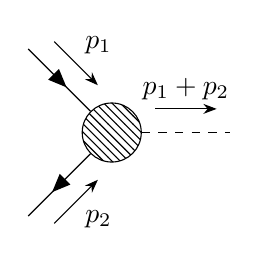
\begin{tikzpicture}[baseline = (b)]
\begin{feynman}
\vertex [blob] (b) {};
\vertex [above left=of b] (a);
\vertex [below left=of b] (c);
\vertex [right=of b] (d);
\diagram* {
(a) -- [fermion, momentum = $p_1$] (b) -- [fermion, rmomentum = $p_2$] (c),
(b) -- [scalar, momentum=$p_1 + p_2$] (d)
};
\end{feynman}
\end{tikzpicture}
 = - i \Gamma(p_1, p_2)
\end{equation*}

\begin{equation*}
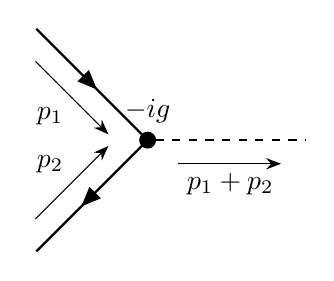
\begin{tikzpicture}[baseline = (a)]
\begin{feynman}[large]
\vertex [dot, label = $-ig$] (a) {};
\vertex [below left=of a] (b);
\vertex [above left=of a] (c);
\vertex [right=of a] (d);
\diagram* {
(a) -- [fermion, rmomentum'=$p_2$] (b),
(c) -- [fermion, momentum'=$p_1$] (a),
(a) -- [scalar, momentum'=$p_1 + p_2$] (d)
};
\end{feynman}
\end{tikzpicture}
\quad
\mathlarger{+}
\quad 	
\feynmandiagram [horizontal = a to b, baseline = (a)] {
	i1 -- [fermion, momentum'=$p_1$] t1 -- [fermion, momentum=$p_1 - k$] a,
	a -- [fermion, rmomentum=$p_2 + k$] t2 -- [fermion, rmomentum'=$p_2$] i2, 
	t1 -- [scalar, momentum'=$k$] t2,
	a -- [scalar, momentum'=$p_1 + p_2$ ] b
	};
\quad
\mathlarger{+}
\quad 	
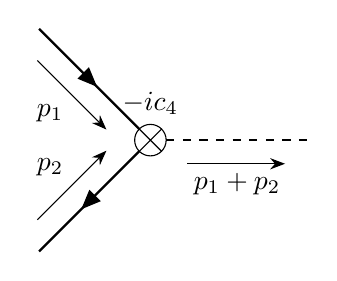
\begin{tikzpicture}[baseline = (a)]
\begin{feynman}[large]
\vertex [crossed dot, label = $-ic_4$] (a) {};
\vertex [below left=of a] (b);
\vertex [above left=of a] (c);
\vertex [right=of a] (d);
\diagram* {
(a) -- [fermion, rmomentum'=$p_2$] (b),
(c) -- [fermion, momentum'=$p_1$] (a),
(a) -- [scalar, momentum'=$p_1 + p_2$] (d)
};
\end{feynman}
\end{tikzpicture}
\end{equation*}
These diagrams represent the amplitudes and main loop integral,
\[ - i \Gamma(p_1, p_2) = (-ig) + (-ig)^3 {\int \frac{\mathrm{d}^4 k}{(2 \pi)^4} \frac{i}{k^2 - M^2 + i \epsilon} \cdot \frac{i (\slashed{p}_1 - \slashed{k} + m)}{(p_1 - k)^2 - m^2 + i \epsilon} \cdot \frac{i (\slashed{p}_2 + \slashed{k} + m)}{(p_2 + k)^2 - m^2 + i \epsilon}} - i c_4	\]
Therefore, we better evaluate this integral, 
\begin{align*}
V(p_1, p_2) =  \int \frac{\mathrm{d}^4 k}{(2 \pi)^4} {\frac{i}{k^2 - M^2 + i \epsilon} \cdot \frac{i (\slashed{p}_1 - \slashed{k} + m)}{(p_1 - k)^2 - m^2 + i \epsilon} \cdot \frac{i (\slashed{p}_2 + \slashed{k} + m)}{(p_2 + k)^2 - m^2 + i \epsilon}}
\end{align*}
First, define the numerator which is an operator which corrects the tree-level vertex operator,
\begin{align*}
N & = {(\slashed{p}_1 - \slashed{k} + m)(\slashed{p}_2 + \slashed{k} + m)} 
\end{align*}
Introducing Feynman parameters and remembering the factor of $(n-1)!$,
\begin{align*}
V(p_1, p_2) & = -2i \int \frac{\mathrm{d}^4 k}{(2 \pi)^4} \int_0^1 \frac{N \d{x} \d{y} \d{z} \delta(x + y + z - 1)}{[x k^2 + y (p_1 - k)^2 + z (p_2 + k)^2 - x M^2 - (y + z) m^2 + i \epsilon]^3}
\\
& = -2i \int \frac{\mathrm{d}^4 k}{(2 \pi)^4} \int_0^1 \frac{N \d{x} \d{y} \d{z} \delta(x + y + z - 1)}{[k^2 - 2 y p_1 \cdot k + y p_1^2 + 2 z p_2 \cdot k + z p_2^2 - x M^2 - (y + z) m^2 + i \epsilon]^3}
\\
& = -2i \int \frac{\mathrm{d}^4 k}{(2 \pi)^4} \int_0^1 \frac{N \d{x} \d{y} \d{z} \delta(x + y + z - 1)}{[(k - yp_1 + z p_2)^2 - (y p_1 - z p_2)^2 + y p_1^2 + z p_2^2 - x M^2 - (y + z) m^2 + i \epsilon]^3}
\\
& = -2i \int \frac{\mathrm{d}^4 \ell}{(2 \pi)^4} \int_0^1 \frac{N \d{x} \d{y} \d{z} \delta(x + y + z - 1)}{[\ell^2 - (y p_1 - z p_2)^2 + y p_1^2 + z p_2^2 - x M^2 - (y + z) m^2 + i \epsilon]^3}
\end{align*}
We must evaluate the numerator in this form with $k = \ell + y p_1 - z p_2$,
\begin{align*}
N & = (\slashed{p}_1(1 - y) + \slashed{p}_2 z - \slashed{\ell} + m)(\slashed{p}_2(1 - z) + \slashed{p}_1 y + \slashed{\ell} + m)
\\
& = (\slashed{p}_1(1 - y) + \slashed{p}_2 z - \slashed{\ell} + m)(\slashed{p}_2(1 - z) + \slashed{p}_1 y + \slashed{\ell} + m) - \ell^2
\\
& = \Delta' - \ell^2
\end{align*}
where linear terms in $\ell$ are dropped because they integrate to zero. Now set,
\[ \Delta = (y p_1 - z p_2)^2 - y p_1^2 - z p_2^2 + x M^2 + (y + z) m^2 - i \epsilon\] 
and perform a Wick rotation $\ell^0 = i \ell_E^0$ so the integral becomes,
\begin{align*}
V(p_1, p_2) & = -2 \int \frac{\mathrm{d}^4 \ell_E}{(2 \pi)^4} \int_0^1 \frac{N \d{x} \d{y} \d{z} \delta(x + y + z - 1)}{[\ell_E^2 + \Delta]^3}
\\
& = - \frac{1}{4 \pi^2} \int_0^1 \d{x} \d{y} \d{z} \delta(x + y + z - 1) \int_{0}^\infty \d{\ell_E} \frac{\Delta' \ell_E^3 + \ell_E^5}{[\ell_E^2 + \Delta]^3}
\end{align*}
The first integral we have seen before and is finite,
\[ \int_{0}^\infty \d{\ell_E} \frac{\ell_E^3}{[\ell_E^2 + \Delta]^3} = \left[ -\frac{2 x^2 + \Delta}{4(x^2 + \Delta)^2} \right]_{0}^\infty = \frac{1}{4 \Delta} \]
However, the second is logarithmically divergent. Mathematica easily evaluates,
\[ \int_0^{\Lambda} \d{\ell_E} \frac{\ell_E^5}{[\ell_E^2 + \Delta]^3} \xrightarrow{\Lambda \to \infty} \frac{1}{2} \left[ \log{\Lambda^2} - \log{\Delta} \right] - \frac{3}{4} \]
Therefore, we can read off the divergence of this diagram,
\[ - i g Z_g = -i g \left( 1 + \frac{g^2}{4 \pi^2} \int_0^1 \d{x} \d{y} \d{z} \delta(x + y + z - 1) \log{\Lambda} + \text{finite} \right) = -i g \left( 1 + \frac{g^2}{8 \pi^2} \log{\Lambda} + \text{finite} \right) \]
Plugging everything together,
\begin{align*}
V(p_1, p_2) = & - \frac{1}{16 \pi^2} \int_0^1 \d{x} \d{y} \d{z} \delta(x + y + z - 1) \frac{(\slashed{p}_1(1 - y) + \slashed{p}_2 z + m)(\slashed{p}_2(1 - z) + \slashed{p}_1 y + m)}{(y p_1 - z p_2)^2 - y p_1^2 - z p_2^2 + x M^2 + (y + z) m^2}
\\
& + \frac{1}{8 \pi^2} \int_0^1 \d{x} \d{y} \d{z} \delta(x + y + z - 1) \log{[(y p_1 - z p_2)^2 - y p_1^2 - z p_2^2 + x M^2 + (y + z) m^2]} 
\end{align*}
where I have already absorbed divergent constants into the counter term. Thus we find,
\begin{align*}
-i \Gamma(p_1, p_2) = & - ig - \frac{i g^3}{16 \pi^2} \int_0^1 \d{x} \d{y} \d{z} \delta(x + y + z - 1) \frac{(\slashed{p}_1(1 - y) + \slashed{p}_2 z + m)(\slashed{p}_2(1 - z) + \slashed{p}_1 y + m)}{(y p_1 - z p_2)^2 - y p_1^2 - z p_2^2 + x M^2 + (y + z) m^2}
\\
& + \frac{i g^3}{8 \pi^2} \int_0^1 \d{x} \d{y} \d{z} \delta(x + y + z - 1) \log{[(y p_1 - z p_2)^2 - y p_1^2 - z p_2^2 + x M^2 + (y + z) m^2]} -  i c_4
\end{align*}
As before we renormalize at some scale $\mu$ by space-like (unphysical) momenta $p_1 = p_2 = (0, \mu, 0, 0)$. Then we find\footnote{I have not subtracted the value of the first term at the renormalization point for convenience. Thus this is not a physical renormalization condition but it will work fine.} , 
\begin{align*}
-i \Gamma(p_1, p_2) = & - i g - \frac{i g^3}{16 \pi^2} \int_0^1 \d{x} \d{y} \d{z} \delta(x + y + z - 1) \frac{(\slashed{p}_1(1 - y) + \slashed{p}_2 z + m)(\slashed{p}_2(1 - z) + \slashed{p}_1 y + m)}{(y p_1 - z p_2)^2 - y p_1^2 - z p_2^2 + x M^2 + (y + z) m^2}
\\
& + \frac{i g^3}{8 \pi^2} \int_0^1 \d{x} \d{y} \d{z} \delta(x + y + z - 1) \log{\left(\frac{(y p_1 - z p_2)^2 - y p_1^2 - z p_2^2 + x M^2 + (y + z) m^2}{-\mu^2(y - z)^2 + (y + z) \mu^2 + x M^2 + (y + z) m^2}\right)}
\end{align*} 
The first term does not produce any running with renormalization scale because, in the limit $\mu \gg m, M$ this term becomes constant in $\mu$ and thus does not have a scale-dependent counter-term. However, the second term produces the logarithmic scaling characteristic of marginal couplings. Taking the limit $\mu \gg m, M$, we can identify the scaling of the vertex function with the scale-dependent term absorbed into the counter term,
\begin{align*}
\deriv{\Gamma}{\mu} = \frac{g^3}{8\pi^2} \int_0^1 \d{x} \d{y} \d{z} \delta(x + y + z - 1) \deriv{}{\mu} \log{[-(y - z)^2 \mu^2 + (y + z) \mu^2]} = \frac{g^3}{8 \pi^2} 
\end{align*}

\subsubsection{The Dressed $\psi$-Propagator}

Again we need the field strength renormalization. However, in the case of marginal coupling we see (consider the above computation or consult Peskin) that only the divergent parts will affect the $\beta$-function in the high-energy limit because only these terms come with logarithmic counter-terms which give the scaling. Here, finite terms produce no scaling. First, consider corrections to the $\psi$ propagator given by the diagrams,
\begin{equation*}
\feynmandiagram [horizontal = a to b, layered layout, baseline = (a)] {
	i1 -- [fermion, momentum'=$p$] a -- [fermion, momentum'=$p - k$] b -- [fermion, momentum'=$p$] f1,
	a -- [scalar, half left, momentum=$k$] b
	};
\quad
\mathlarger{+}
\quad 	
\feynmandiagram [horizontal = a to b, layered layout, baseline = (a)] {
	i1 -- [fermion, momentum'=$p$] a [crossed dot, label = \(- i c_2 - i \slashed{p} c_6 \)] -- [fermion, momentum'=$p$] b
	};	
\end{equation*}
The loop integral we need in then,
\begin{align*}
V(p) & = (-i g)^2 \int \frac{\dn{4}{k}}{(2 \pi)^4} \frac{i(\slashed{p} - \slashed{k} + m)}{(p-k)^2 - m^2 + i \epsilon} \cdot \frac{i}{k^2 - M^2 + i \epsilon}
\\
& = g^2 \int \frac{\dn{4}{k}}{(2 \pi)^4} \int_0^1 \d{x} \frac{(\slashed{p} - \slashed{k} + m)}{[x (p-k)^2 + (1 - x) k^2 - x m^2 - (1 - x) M^2 + i \epsilon]^2}
\\
& = g^2 \int \frac{\dn{4}{k}}{(2 \pi)^4} \int_0^1 \d{x} \frac{(\slashed{p} - \slashed{k} + m)}{[k^2 + x p^2 - 2 x p \cdot k - x m^2 - (1 - x) M^2 + i \epsilon]^2}
\\
& = g^2 \int \frac{\dn{4}{k}}{(2 \pi)^4} \int_0^1 \d{x} \frac{(\slashed{p} - \slashed{k} + m)}{[(k - x p)^2 + x(1 - x) p^2  - x m^2 - (1 - x) M^2 + i \epsilon]^2} 
\end{align*}
Now we take $\ell = k - x p$ and write,
\begin{align*}
V(p) & = g^2 \int \frac{\dn{4}{\ell}}{(2 \pi)^4} \int_0^1 \d{x} \frac{(\slashed{p} (1 - x) - \slashed{\ell} + m)}{[\ell^2 + x(1 - x) p^2  - x m^2 - (1 - x) M^2 + i \epsilon]^2} 
\end{align*}
we can immediately drop the linear $\ell$ term in the numerator to get, 
\begin{align*}
V(p) & = g^2  \int_0^1 \d{x} \int \frac{\dn{4}{\ell}}{(2 \pi)^4} \frac{(1 - x) \slashed{p} + m}{[\ell^2 + x(1 - x) p^2  - x m^2 - (1 - x) M^2 + i \epsilon]^2} 
\end{align*}
The integral over $\ell$ is identical to in the scalar field case giving,
\begin{align*}
V(p) & = - \frac{ig^2}{16 \pi^2} \left[ \int_0^1 \d{x} ((1 - x) \slashed{p} + m) \left( \log{\left[ x(x - 1) p^2  + x m^2 + (1 - x) M^2 \right] } + \text{divergent constants} \right) \right] 
\end{align*}
The counter-terms have exactly the correct form to cancel the divergent quantity multiplied by $\tfrac{1}{2} \slashed{p} + m$. Therefore,
\[ \Sigma_\psi(p) = \frac{g^2}{16 \pi^2} \left[ \int_0^1 \d{x} ((1 - x) \slashed{p} + m)  \log{\left[ x(x - 1) p^2  + x m^2 + (1 - x) M^2 \right] }  \right] + \text{counter terms} \]
This expression allows us to easily identify the change in the field strength renormalization in the high energy limit as the scale-dependent term going into the counter-term $c_6$ which gives,
\[ \deriv{\log{Z_{\psi}}}{\log{\mu}} = \frac{g^2}{16 \pi^2} \int_0^1 (1 - x) \deriv{}{\mu} \log{[x(1-x) \mu^2]} =  \frac{g^2}{16 \pi^2} \]

\subsubsection{The Dressed $\phi$-Propagator}

At the one-loop level, there are exactly two diagrams which contribute to the renormalization of the $\phi$ propagator,
\begin{equation*}
\feynmandiagram [horizontal = a to b, layered layout, baseline = (a)] {
	i1 -- [scalar, momentum'=$p$] a -- [fermion, half right, momentum'=$p + k$] b -- [scalar, momentum'=$p$] f1,
	b -- [fermion, half right, momentum'=$k$] a
	};
\quad
\mathlarger{+}
\quad 	
\feynmandiagram [horizontal = a to b, layered layout, baseline = (a)] {
	i1 -- [scalar, momentum'=$p$] a [crossed dot, label = \(- i c_3 - i p^2 c_5\)] -- [scalar, momentum'=$p$] b
	};	
\end{equation*} 
We first evaluate the loop integral remembering the minus due to fermion loops,
\begin{align*}
V(p) & = - (- i g)^2 \tr{\int \frac{\dn{4}{k}}{(2 \pi)^4} \frac{i (\slashed{k} + m)}{k^2 - m^2 + i \epsilon} \cdot \frac{i (\slashed{p} + \slashed{k} + m)}{(p + k)^2 - m^2 + i \epsilon}}
\\
& = - g^2 \int \frac{\dn{4}{k}}{(2 \pi)^4} \int_0^1 \d{x} \tr{ \frac{ (\slashed{k} + m) (\slashed{p} + \slashed{k} + m)}{[k^2 + 2 x p \cdot k + x p^2 - m^2 + i \epsilon]^2}}
\\
& = - g^2 \int \frac{\dn{4}{k}}{(2 \pi)^4} \int_0^1 \d{x} \tr{\frac{ (\slashed{k} + m) (\slashed{p} + \slashed{k} + m)}{[(k + x p)^2 + x(1 - x) p^2 - m^2 + i \epsilon]^2}}
\end{align*}
Now take $\ell = k + x p$ and then expand dropping linear terms in $\ell$ which integrate out,
\begin{align*}
V(p) & =  - g^2 \int \frac{\dn{4}{\ell}}{(2 \pi)^4} \int_0^1 \d{x} \tr{\frac{ (\slashed{\ell} - x \slashed{p} + m) ((1 - x)\slashed{p} + \slashed{\ell} + m)}{[\ell^2 + x(1 - x) p^2 - m^2 + i \epsilon]^2}}
\\
& =  - g^2 \int \frac{\dn{4}{\ell}}{(2 \pi)^4} \int_0^1 \d{x} \tr{\frac{\ell^2 - (x \slashed{p} - m) ((1 - x)\slashed{p} + m)}{[\ell^2 + x(1 - x) p^2 - m^2 + i \epsilon]^2}}
\end{align*}
Now consider,
\begin{align*}
\tr{(x \slashed{p} - m) ((1 - x)\slashed{p} + m)} & = \tr{x \slashed{p} (1 - x) \slashed{p}} - m (1 - x) \tr{\slashed{p}} + x \tr{\slashed{p}} m - \tr{m^2} 
\\
& = 4 x(1 - x) p^2 - 4 m^2
\end{align*}
Thus,
\begin{align*}
V(p) 
& =  - 4g^2 \int \frac{\dn{4}{\ell}}{(2 \pi)^4} \int_0^1 \d{x} \frac{\ell^2 + x(x - 1) p^2 + m^2}{[\ell^2 + x(1 - x) p^2 - m^2 + i \epsilon]^2}
\end{align*}
Wick rotating and performing the integral over $\ell$ we have two divergent integrals one extremely badly divergent. Splitting the term into two integral and recognizing that this first integral is identical to in the scalar case,
\begin{align*}
V_1(p) & = - 4g^2 \int_0^1 \frac{\dn{4}{\ell}}{(2 \pi)^4} \int_0^1 \d{x} \frac{x(x - 1) p^2 + m^2}{[\ell^2 + x(1 - x) p^2 - m^2 + i \epsilon]^2}
\\
& = \frac{ig^2}{4 \pi^2} \int \d{x} [x(x - 1) p^2 + m^2]\left(  \log{[x(x - 1) p^2 + m^2]} + \text{divergent junk} \right)
\end{align*}
Again the counter term has the exact correct form to cancel the momentum dependence of the divergence. The second integral will need a bit more work.
\begin{align*}
V_2(p) & = - 4g^2 \int \frac{\dn{4}{\ell}}{(2 \pi)^4} \int_0^1 \d{x} \frac{\ell^2}{[\ell^2 + x(1 - x) p^2 - m^2 + i \epsilon]^2}
\\
& = 4i g^2 \int \frac{\dn{4}{\ell_E}}{(2 \pi)^4} \int_0^1 \d{x} \frac{\ell_E^2}{[\ell_E^2 - x(1 - x) p^2 + m^2 + i \epsilon]^2}
\\
& = \frac{ig^2}{2 \pi^2}  \int_0^1 \d{x} \int \d{\ell_E} \frac{\ell_E^5}{[\ell_E^2 - x(1 - x) p^2 + m^2 + i \epsilon]^2}
\\
& = \frac{ig^2}{2 \pi^2} \left[ \int_0^1 \d{x} [x(x - 1)p^2 + m^2] \left( \frac{1}{2} + \log{[x(x - 1)p^2 + m^2]} - \log{\Lambda^2} \right) + \tfrac{1}{2} \Lambda^2 \right]
\end{align*}
And again he counter term has the exact correct form to cancel the momentum dependence of the divergence.
Therefore,
\begin{align*}
\Sigma_\phi(p) = & - \frac{3g^2}{4 \pi^2} \int_0^1 \d{x} [x(x - 1)p^2 + m^2] \log{[x(x - 1)p^2 + m^2]} + \text{const c.t.}
\end{align*}
As before, these expressions allow us to easily identify the change in the field strength renormalization in the high energy limit as the scale-dependent term going into the counter-term $c_5$ i.e. the part proportional to $p^2$. This gives,
\[ \deriv{\log{Z_{\phi}}}{\log{\mu}} = - \frac{3g^2}{4 \pi^2} \int_0^1 \d{x} x(x - 1) \deriv{}{\mu} \log{[x(1 - x)\mu^2]} = - \frac{3g^2}{2 \pi^2} \int_0^1 \d{x} x(x - 1) = \frac{g^2}{4 \pi^2} \]

\subsubsection{The RG Flow}

We have seen from the Callan-Symanzik equation that,
\[ \beta(g) = \deriv{\Gamma}{\log{\mu}} + g \deriv{\log{Z_{\psi}}}{\log{\mu}} + \frac{1}{2} g \deriv{\log{Z_{\phi}}}{\log{\mu}} \]
Therefore, plugging in,
\[ \beta(g) = \frac{g^3}{8\pi^2} + \frac{g^3}{16 \pi^2} + \frac{g^3}{8 \pi^2} = \frac{5 g^3}{16\pi^2} 
\]
We recover the classic value of the Yukawa theory $\beta$-function. Since the coupling $g$ is marginal, the RG flow takes the standard form of logarithmic running.  

\subsection{Quartic Fermionic Theory} 

Suppose we take the limit $M \to \infty$ of the previous s Fermionic Yukawa theory as the mass of the scalar meson goes to infinity. Consider the path-integral for this theory,
\[ Z = \int \pathd{\bar{\psi}} \pathd{\psi} \pathd{\phi} \exp{\left( i \int \dn{4}{x} \left[ \tfrac{1}{2} \partial_\mu \phi \partial^\mu \phi - \tfrac{1}{2} M^2 \phi^2 + \bar{\psi} (i \slashed{\partial} - m)\psi - g \bar{\psi} \psi \phi  \right] \right)} \]
Now define an auxiliary field $\sigma = M \phi$ which we will hold fixed in the limit $M \to \infty$. Integrating out the $\sigma$ field,
\begin{align*}
Z & = \int \pathd{\bar{\psi}} \pathd{\psi} \pathd{\sigma} \exp{\left( i \int \dn{4}{x} \left[ \tfrac{1}{2} M^{-2} \partial_\mu \sigma \partial^\mu \sigma - \tfrac{1}{2} \sigma^2 + \bar{\psi} (i \slashed{\partial} - m)\psi - \tfrac{g}{M} \sigma \bar{\psi} \psi   \right] \right)}
\\
& = \int \pathd{\bar{\psi}} \pathd{\psi} \pathd{\sigma} \exp{\left( i \int \dn{4}{x} \left[ \tfrac{1}{2} M^{-2} \partial_\mu \sigma \partial^\mu \sigma + \bar{\psi} (i \slashed{\partial} - m)\psi - \tfrac{1}{2} (\sigma + \tfrac{g}{M} \bar{\psi} \psi)^2 + \tfrac{g^2}{2M^2} (\bar{\psi} \psi)(\bar{\psi} \psi) \right] \right)}
\\
& \approx \int \pathd{\bar{\psi}} \pathd{\psi} \pathd{\sigma} \exp{\left( i \int \dn{4}{x} \left[ - \tfrac{1}{2} (\sigma + \tfrac{g}{M} \bar{\psi} \psi)^2 + \bar{\psi} (i \slashed{\partial} - m)\psi + \tfrac{g^2}{2M^2} (\bar{\psi} \psi)(\bar{\psi} \psi) \right] \right)}
\\
& = \int \pathd{\bar{\psi}} \pathd{\psi} \det{[-\tfrac{1}{2}]} \exp{\left( i \int \dn{4}{x} \left[ \bar{\psi} (i \slashed{\partial} - m)\psi + \tfrac{g^2}{2M^2} (\bar{\psi} \psi) (\bar{\psi} \psi)   \right] \right)}
\end{align*}
Therefore, up to an overall constant\footnote{Because $\sigma$ has no kinetic terms in the limit $M \to \infty$ there is no coupling introduced in the functional determinant; it is simply a constant which does not effect any observable.}, this theory is formally equivalent in the $M \to \infty$ limit to a theory of fermions with quartic interactions,
\[ \lagrange = \bar{\psi} (i \slashed{\partial} - m)\psi + \tfrac{g^2}{2M^2} (\bar{\psi} \psi) (\bar{\psi} \psi)  \]
We define $\lambda = \left(\frac{g}{M}\right)^2$. 

\subsubsection{Calculations in Effective Field Theory}

We consider the diagrams corresponding to $\psi \bar{\psi} \mapsto \psi \bar{\psi}$ scattering at one-loop which is given by the Feynman diagrams,
\begin{equation*}
\feynmandiagram [vertical=i1 to f2, baseline = (c)][ edges={fermion}] {
  {i1, i2} -- c [dot] -- {f1, f2},
};
\quad
\mathlarger{+}
\quad 	
\feynmandiagram [layered layout, horizontal= a to b, baseline = (a)] [edges=fermion] {
i1 -- a -- [half left] b -- [half left] a,
b -- f1,
a -- i2,
f2 -- b
};
\quad
\mathlarger{+}
\quad 	
\feynmandiagram [layered layout, vertical=b to a, baseline = 1.7cm] [edges=fermion] {
i1 -- a -- [half left] b -- [half left] a,
b -- f2,
a -- i2,
f1 -- b
};
+
\feynmandiagram [vertical=i1 to f2, baseline = (c)][ edges={fermion}] {
  {i1, i2} -- c [crossed dot] -- {f1, f2},
};
\end{equation*}
Thankfully we have already computed this fermionic loop integral so there is very little work to be done. These diagrams give the amplitude (with external leg spinor factors amputated), 
\begin{align*}
i \mathcal{M} = i \lambda + V(t) - V(t) + i c_\lambda 
\end{align*}
in which we mus remember the relative minus sign due to Fermion order swapping and we have defined,
\begin{align*}
V(q^2) = & \frac{i\lambda^2}{4 \pi^2} \left[ \int_0^1 \d{x} [x(x - 1) p^2 + m^2]\left(  3 \log{[x(x - 1) p^2 + m^2]} - 3 \log{\Lambda^2} + 2 \right) + \tfrac{1}{2} \Lambda^2 \right]
\end{align*}
The quadratically divergent term is absorbed by $c_{\lambda}$ making a constant shift of the coupling constant strength.
And as usual we remove the logarithmic divergences into our counter-terms ... oh wait! The divergences carry factors of the momentum but there are now such four valent vertices in our theory which can possibly cancel this very bad momentum dependent divergence. We should have expected this from the start since the coupling $\lambda = \left( \frac{g}{M} \right)^2$ has negative mass dimension and quartic fermion interaction like Fermi's theory of solids are famously non-renormalizable. To cancel such divergences requires the generation of higher-order interaction terms in dimension and derivative expansions such as,
\[ g' M^{-4} ( \partial_\mu \bar{\psi} \partial^\mu \psi) (\bar{\psi} \psi) +  g' M^{-4} \partial_\mu \bar{\psi} \psi (\partial^\mu \bar{\psi} \psi) + g' M^{-4} \bar{\psi}  \partial_\mu \psi (\bar{\psi} \partial^\mu \psi) \]
Such terms give an additional vertex diagram which   couple momenta on the incoming and outgoing legs. Such terms can a general contribution of,
\[  i g' M^{-4} \left( p_1 + p_2 \right) \cdot \left( p_2 + p_4 \right) - i g' M^{-4} \left( p_1 - p_3 \right) \left( p_2 - p_4 \right) = i g' M^{-4} \: (s - t) \]
This is exactly the correct form to cancel the momentum dependent divergences at the scale $\mu$ if we take,
\[ g' = \frac{\lambda^2 M^4}{4 \pi^2} \int_0^1 x(x  - 1) \left[ 3 \log{\Lambda^2} - 2 - 3 \log{(x(1 - x) \mu^2 + m^2)} \right] \]
and the counter term,
\[ c_{\lambda} = \frac{\lambda^2}{4 \pi^2} \left[ \int_0^1 m^2 \left( 3 \log{\Lambda^2} - 2 - 3 \log{(x(1 - x) \mu^2 + m^2)} \right) - \tfrac{1}{2} \Lambda^2 \right] \]

\subsubsection{The RG Flow}

Because there are no one-loop two-valent 1PI diagrams in the quartic theory, there is thankfully no field strength renormalization at this level of perturbation theory. Therefore, we can read off the ruining of couplings from this theory. We find (remembering to perform the integral $\int_0^1 \d{x} x(x-1) = - \frac{1}{6}$ for the $g'$ coupling),
\begin{align*}
\deriv{\lambda}{\log{\mu}} & = -\frac{3 \lambda^2 m^2}{2 \pi^2}
\\
\deriv{g'}{\log{\mu}} & = \frac{\lambda^2 M^4}{4 \pi^2}
\end{align*}
Therefore, we find that a nonzero coupling $\lambda$ will automatically generate growing $g'$ terms as the theory flows into the UV. Intriguingly, the $\beta$-function for $\lambda$ is negative and small (assuming that $m \ll M$) meaning that the coupling $\lambda$ decreases slowly into the UV. I am not quite certain of the interpretation of this. Note that unlike the scalar Yukawa theory, we already have well-behaved $\beta$ functions for dimensionful parameters. This is because there is a natural dimensionful scale of the theory, namely $M$, which appears in the $\beta$-function instead of explicit factors of the renormalization scale. It will be somewhat illuminating to express these RG flow equations in terms of the microscopic marginal Yukawa coupling $g$. We find,
\begin{align*}
\deriv{g^2}{\log{\mu}} = - \frac{3 g^4 m^2}{2 \pi^2 M^2}
\end{align*} 
which implies that,
\begin{align*}
\deriv{g}{\log{\mu}} = - \frac{3 g^3}{4 \pi^2} \left( \frac{m}{M} \right)^2 
\end{align*} 
Note that the expansion parameter $\frac{m}{M}$ appears explicitly in the $\beta$-function. 
Furthermore, we have,
\begin{align*}
\deriv{g'}{\log{\mu}} = \frac{g^4}{4 \pi^2}
\end{align*}
This theory is equivalent to the previous Yukawa theory we considered as formal power expansion in $\frac{m}{M}$. However, we see that the couplings evolve differently in the quartic theory. In the quartic theory, logarithmic running of the marginal coupling is suppressed and its effect is dumped into generating higher-order interaction vertices. Because Yukawa theory is renormalizable, the RG flow can be tuned to remain in the stable subspace of renormalizable couplings. However, the quartic theory is guaranteed, as we have seen, to generate growing couplings of all orders as we flow from IR to UV. However, these theories are still equivalent in the sense of Wilsonian RG. Both theories are guaranteed to flow to a finite-dimensional stable subspace parameterized by renormalizable couplings in the IR. Then path-integral arguments show exactly the equivalence mapping between such subspaces of couplings even though the quartic interaction does still generate these non-renormalizable couplings as expected in the Wilsonian RG.

\subsubsection{Generation of Higher-Order Interactions}

We showed in class how higher-order interactions in dimension and derivative expansion need to be included in the Lagrangian to diagrammatically match the effective field theory of a heavy Yukawa  interaction. Here, we will investigate the generation of such terms in a little more depth. Consider again the path integral for the massive Yukawa theory,
\begin{align*}
Z 
& = \int \pathd{\bar{\psi}} \pathd{\psi} \pathd{\sigma} \exp{\left( i \int \dn{4}{x} \left[ \tfrac{1}{2} M^{-2} \partial_\mu \sigma \partial^\mu \sigma - \tfrac{1}{2} (\sigma + \tfrac{g}{M} \bar{\psi} \psi)^2 + \bar{\psi} (i \slashed{\partial} - m)\psi  + \tfrac{g^2}{2M^2} (\bar{\psi} \psi)(\bar{\psi} \psi) \right] \right)}
\end{align*}
Define a new auxiliary field, $\tilde{\sigma} = \sigma + \tfrac{g}{M} \bar{\psi} \psi$. Then we have,
\begin{align*}
Z & = \int \pathd{\bar{\psi}} \pathd{\psi} \pathd{\tilde{\sigma}} \exp{\left( i \int \dn{4}{x} \left[ \tfrac{1}{2} M^{-2} \partial_\mu (\tilde{\sigma}  - \tfrac{g}{M} \bar{\psi} \psi) \partial^\mu (\tilde{\sigma} - \tfrac{g}{M} \bar{\psi} \psi) - \tfrac{1}{2} \tilde{\sigma}^2 + \bar{\psi} (i \slashed{\partial} - m)\psi + \tfrac{g^2}{2M^2} (\bar{\psi} \psi)(\bar{\psi} \psi) \right] \right)}
\end{align*}
Expanding this effective Lagrangian,
\begin{align*}
\lagrange_{\text{eff}} & = \tfrac{1}{2} M^{-2} \partial_\mu (\tilde{\sigma}  - \tfrac{g}{M} \bar{\psi} \psi) \partial^\mu (\tilde{\sigma} - \tfrac{g}{M} \bar{\psi} \psi) - \tfrac{1}{2} \tilde{\sigma}^2 + \bar{\psi} (i \slashed{\partial} - m)\psi + \tfrac{g^2}{2M^2} (\bar{\psi} \psi)(\bar{\psi} \psi)
\\
& = \tfrac{1}{2M^2} \partial_\mu \tilde{\sigma} \partial^\mu \tilde{\sigma} - \tfrac{g}{M^3} \partial_\mu \tilde{\sigma} \partial^\mu (\bar{\psi} \psi) + \tfrac{g^2}{2M^4} \partial_\mu (\bar{\psi} \psi) \partial^\mu (\bar{\psi} \psi) - \tfrac{1}{2} \tilde{\sigma}^2 + \bar{\psi} (i \slashed{\partial} - m)\psi + \tfrac{g^2}{2M^2} (\bar{\psi} \psi)(\bar{\psi} \psi)
\end{align*}
Then integrating the second term by parts we get,
\begin{align*}
\lagrange_{\text{eff}} 
& = \tfrac{1}{2M^2} \partial_\mu \tilde{\sigma} \partial^\mu \tilde{\sigma} + \tfrac{g}{M^3} \tilde{\sigma} \partial_\mu  \partial^\mu (\bar{\psi} \psi) + \tfrac{g^2}{2M^4} \partial_\mu (\bar{\psi} \psi) \partial^\mu (\bar{\psi} \psi) - \tfrac{1}{2} \tilde{\sigma}^2 + \bar{\psi} (i \slashed{\partial} - m)\psi + \tfrac{g^2}{2M^2} (\bar{\psi} \psi)(\bar{\psi} \psi)
\end{align*}
Again completing the square we find,
\begin{align*}
\lagrange_{\text{eff}} 
& = \tfrac{1}{2M^2} \partial_\mu \tilde{\sigma} \partial^\mu \tilde{\sigma} - \tfrac{1}{2} (\tilde{\sigma} - \tfrac{g}{M^3} \partial^2 (\bar{\psi} \psi) )^2 
+ \bar{\psi} (i \slashed{\partial} - m)\psi + \tfrac{g^2}{2M^2} (\bar{\psi} \psi)(\bar{\psi} \psi) + \tfrac{g^2}{2M^4} \partial_\mu (\bar{\psi} \psi) \partial^\mu (\bar{\psi} \psi) + \tfrac{g^2}{2M^6} [\partial^2 (\bar{\psi} \psi)]^2 
\end{align*}
At this point we change variables again to $\tilde{\tilde{\sigma}} = \tilde{\sigma} - \tfrac{g}{M^3} \partial^2 (\bar{\psi} \psi)$ which now only differs from $\tilde{\sigma}$ by a term of order $M^{-3}$ rather than the term of order $M^{-1}$ between $\tilde{\sigma}$ and $\sigma$. Then we have, 
\begin{align*}
\lagrange_{\text{eff}} 
& = \tfrac{1}{2M^2} \partial_\mu \tilde{\sigma} \partial^\mu \tilde{\sigma} - \tfrac{1}{2} \tilde{\tilde{\sigma}}^2 
+ \bar{\psi} (i \slashed{\partial} - m)\psi + \tfrac{g^2}{2M^2} (\bar{\psi} \psi)(\bar{\psi} \psi) + \tfrac{g^2}{2M^4} \partial_\mu (\bar{\psi} \psi) \partial^\mu (\bar{\psi} \psi) + \tfrac{g^2}{2M^6} [\partial^2 (\bar{\psi} \psi)]^2 
\end{align*}
We may repeat this process ad-infinitum to generate the sequence of Lorentz-invariant derivative couplings. However, since our change of variables is at order $M^{-3}$ we may wish to integrate out the $\sigma$ field at this level to find the effective field theory up to order $M^{-3}$. Since $\tilde{\sigma}$ is shifted from the integration variables by a quantity of order $M^{-3}$ we are justified in ignoring the kinetic term which would, in actuality, be corrected due to its spatial dependence on $\bar{\psi} \psi$. If we drop this term, then we have, 
\begin{align*}
Z = \int \pathd{\bar{\psi}} \pathd{\psi} & \pathd{\tilde{\sigma}}
\\
& \exp{\left( i \int \dn{4}{x} \left[ - \tfrac{1}{2} \tilde{\tilde{\sigma}}^2 
+ \bar{\psi} (i \slashed{\partial} - m)\psi + \tfrac{g^2}{2M^2} (\bar{\psi} \psi)(\bar{\psi} \psi) + \tfrac{g^2}{2M^4} \partial_\mu (\bar{\psi} \psi) \partial^\mu (\bar{\psi} \psi) + \tfrac{g^2}{2M^6} [\partial^2 (\bar{\psi} \psi)]^2 \right] \right)}
\end{align*}
from which we can trivially integrate out $\tilde{\tilde{\sigma}}$ to find, up to a constant,
\begin{align*}
Z & = \int \pathd{\bar{\psi}} \pathd{\psi} \exp{\left( i \int \dn{4}{x} \left[ \bar{\psi} (i \slashed{\partial} - m)\psi + \tfrac{g^2}{2M^2} (\bar{\psi} \psi)(\bar{\psi} \psi) + \tfrac{g^2}{2M^4} \partial_\mu (\bar{\psi} \psi) \partial^\mu (\bar{\psi} \psi) + \tfrac{g^2}{2M^6} [\partial^2 (\bar{\psi} \psi)]^2 \right] \right)}
\end{align*}
Thus we have generated exactly the term,
\[ tfrac{g^2}{2M^4} \partial_\mu (\bar{\psi} \psi) \partial^\mu (\bar{\psi} \psi) \]
required to define renormalized perturbation theory consistently. Furthermore, we have generated an order $M^{-6}$ term
\[ \tfrac{g^2}{2M^6} [\partial^2 (\bar{\psi} \psi)]^2 \]
which is couples momenta at order $p^4$ in a manifestly Lorentz-invariant interaction. 
\end{document}